\documentclass[hyperref={pdfpagelabels=true}]{beamer}
\usepackage{lmodern}
\usepackage{textpos}
\usepackage{amsmath}
\usepackage{tcolorbox}
\usepackage{graphicx,xcolor}
\usepackage{listings}
\usepackage{pifont}
\usepackage{booktabs}% http://ctan.org/pkg/booktabs
\usepackage[final]{pdfpages}
\usepackage{multimedia}
\usepackage{attachfile}
\usepackage{media9}


%\attachfile{\jobname.tex}
%%----------------attach using embedfile-----------------------------------
\usepackage{embedfile}
%\immediate\write18{zip -j -e -P mypassword -r \jobname.tex.zeep \jobname.tex}
%\embedfile{\jobname.tex}
%%----------------attach using navigator-----------------------------------
\usepackage{navigator}
\usepackage{color} %red, mygreen, blue, yellow, cyan, magenta, black, white
\definecolor{mygreen}{RGB}{28,172,0} % color values Red, mygreen, Blue
\definecolor{mygree}{RGB}{95,135,185} % color values Red, mygreen, Blue
\definecolor{mylilas}{RGB}{170,55,241}
\usepackage[utf8]{inputenc} % UFT8 - danske bogstaver
\usepackage[T1]{fontenc}
\usepackage[version=3]{mhchem}
\usepackage{tikz}
\usetikzlibrary{matrix,shapes,arrows,positioning,chains}
%\usepackage{xcolor}
\usepackage{xparse}
\usepackage{xmpmulti}
\usetikzlibrary{shapes.geometric, arrows}
\usetikzlibrary{shapes,snakes}
\usetikzlibrary{chains,fit,shapes}
\usepackage{amssymb}
\usepackage{ifthen}
\usepackage{animate}
\usetikzlibrary{shapes,arrows}
\usepackage{amsmath,bm,times}
\usetikzlibrary[topaths]
\usetikzlibrary{decorations.pathmorphing} % noisy shapes
\usetikzlibrary{fit}					% fitting shapes to coordinates
\usetikzlibrary{backgrounds}	% drawing the background after the foreground
\usepackage{lipsum}   % To generate test text
\usepackage{framed}
\usepackage{ifthen}
\usepackage{geometry}% for screen preview
\sloppy
\definecolor{lightgray}{gray}{0.5}
\setlength{\parindent}{0pt}
\usepackage{amsthm}
\usepackage{amsfonts}
\usetikzlibrary{decorations.pathmorphing,calc,shadows.blur,shadings}

\newcounter{mathseed}
\setcounter{mathseed}{3}
\pgfmathsetseed{\arabic{mathseed}} % To have predictable results
% Define a background layer, in which the parchment shape is drawn
\pgfdeclarelayer{background}
\pgfsetlayers{background,main}

% This is the base for the fractal decoration. It takes a random point between the start and end, and
% raises it a random amount, thus transforming a segment into two, connected at that raised point
% This decoration can be applied again to each one of the resulting segments and so on, in a similar
% way of a Koch snowflake.
\pgfdeclaredecoration{irregular fractal line}{init}
{
  \state{init}[width=\pgfdecoratedinputsegmentremainingdistance]
  {
    \pgfpathlineto{\pgfpoint{random*\pgfdecoratedinputsegmentremainingdistance}{(random*\pgfdecorationsegmentamplitude-0.02)*\pgfdecoratedinputsegmentremainingdistance}}
    \pgfpathlineto{\pgfpoint{\pgfdecoratedinputsegmentremainingdistance}{0pt}}
  }
}


% define some styles
\tikzset{
   paper/.style={draw=black!10, blur shadow, every shadow/.style={opacity=1, black}, shading=bilinear interpolation,
                 lower left=black!10, upper left=black!5, upper right=white, lower right=black!5, fill=none},
   irregular cloudy border/.style={decoration={irregular fractal line, amplitude=0.2},
           decorate,
     },
   irregular spiky border/.style={decoration={irregular fractal line, amplitude=-0.2},
           decorate,
     },
   ragged border/.style={ decoration={random steps, segment length=7mm, amplitude=2mm},
           decorate,
   }
}

\def\tornpaper#1{%
\ifthenelse{\isodd{\value{mathseed}}}{%
\tikz{
  \node[inner sep=1em] (A) {#1};  % Draw the text of the node
  \begin{pgfonlayer}{background}  % Draw the shape behind
  \fill[paper] % recursively decorate the bottom border
     \pgfextra{\pgfmathsetseed{\arabic{mathseed}}\addtocounter{mathseed}{1}}%
      {decorate[irregular cloudy border]{decorate{decorate{decorate{decorate[ragged border]{
        (A.north west) -- (A.north east)
      }}}}}}
      -- (A.south east)
     \pgfextra{\pgfmathsetseed{\arabic{mathseed}}}%
      {decorate[irregular spiky border]{decorate{decorate{decorate{decorate[ragged border]{
      -- (A.south west)
      }}}}}}
      -- (A.north west);
  \end{pgfonlayer}}
}{%
\tikz{
  \node[inner sep=1em] (A) {#1};  % Draw the text of the node
  \begin{pgfonlayer}{background}  % Draw the shape behind
  \fill[paper] % recursively decorate the bottom border
     \pgfextra{\pgfmathsetseed{\arabic{mathseed}}\addtocounter{mathseed}{1}}%
      {decorate[irregular spiky border]{decorate{decorate{decorate{decorate[ragged border]{
        (A.north east) -- (A.north west)
      }}}}}}
      -- (A.south west)
     \pgfextra{\pgfmathsetseed{\arabic{mathseed}}}%
      {decorate[irregular cloudy border]{decorate{decorate{decorate{decorate[ragged border]{
      -- (A.south east)
      }}}}}}
      -- (A.north east);
  \end{pgfonlayer}}
}}
% A counter, since TikZ is not clever enough (yet) to handle
% arbitrary angle systems.
\newcount\mycount
%\usepackage{asymptote}
\newcommand{\mx}[1]{\mathbf{\bm{#1}}} % Matrix command
\newcommand{\vc}[1]{\mathbf{\bm{#1}}} % Vector command
\newcounter{angle}
\setcounter{angle}{0}

\usetheme[hideothersubsections]{Hannover}
\usecolortheme{dove,sidebartab}

%\useoutertheme{infolines}

\definecolor{mygray}{gray}{0.6}

\tikzstyle{mybox1} = [draw=red, fill=blue!20, very thick,
    rectangle, rounded corners, inner sep=10pt, inner ysep=10pt]
\tikzstyle{fancytitle1} =[fill=red, text=white]


\tikzstyle{mybox2} = [draw=mygreen, fill=gray!20, very thick,
    rectangle, rounded corners, inner sep=10pt, inner ysep=10pt]
\tikzstyle{fancytitle2} =[fill=mygreen, text=white]

\tikzstyle{mybox} = [draw=blue, fill=green!20, very thick,
    rectangle, rounded corners, inner sep=10pt, inner ysep=20pt]
\tikzstyle{fancytitle} =[fill=blue, text=white, ellipse]

\tikzstyle{startstop} = [rectangle, rounded corners, minimum width=3cm, minimum height=1cm,text centered, draw=black, fill=red!30]
\tikzstyle{io} = [trapezium, trapezium left angle=70, trapezium right angle=110, minimum width=3cm, minimum height=1cm, text centered, draw=black, fill=blue!30]
\tikzstyle{process} = [rectangle, minimum width=3cm, minimum height=1cm, text centered, draw=black, fill=orange!30]
\tikzstyle{decision} = [diamond, minimum width=3cm, minimum height=1cm, text centered, draw=black, fill=green!30]
\tikzstyle{arrow} = [thick,->,>=stealth]

\NewDocumentCommand{\framecolorbox}{oommm}
 {% #1 = width (optional)
  % #2 = inner alignment (optional)
  % #3 = frame color
  % #4 = background color
  % #5 = text
  \IfValueTF{#1}
   {%
    \IfValueTF{#2}
     {\fcolorbox{#3}{#4}{\makebox[#1][#2]{#5}}}
     {\fcolorbox{#3}{#4}{\makebox[#1]{#5}}}%
   }
   {\fcolorbox{#3}{#4}{#5}}%
 }
%\usepackage{animate}

\def\swidth{2.2cm}
\setbeamersize{sidebar width left=\swidth}
\setbeamertemplate{sidebar left}
{
  {\usebeamerfont{title in sidebar}%
    \vskip1.5em%
    \usebeamercolor[fg]{title in sidebar}%
    \insertshorttitle[width=\swidth,center,respectlinebreaks]\par%
    \vskip1.25em%
  }%
  {%
    \usebeamercolor[fg]{author in sidebar}%
    \usebeamerfont{author in sidebar}%
    \insertshortauthor[width=\swidth,center,respectlinebreaks]\par%
        \vskip1.25em%
      }%
      \hbox to2cm{\hss\insertlogo\hss}
      \vskip1.25em%
      \insertverticalnavigation{\swidth}%
      \vfill
      \hbox to2cm{\hskip0.6cm\usebeamerfont{subsection in
          sidebar}\strut\usebeamercolor[fg]{subsection in
          sidebar}\insertframenumber/\inserttotalframenumber\hfill}%
      \vskip3pt%
}%

\mode<presentation>
{
  \usetheme[hideothersubsections]{Hannover}%{CambridgeUS}%
  \setbeamercovered{transparent}
}

%\setbeamertemplate{footline}[frame number]
%\useoutertheme{infolines}
%\setbeamertemplate{headline}{}\setbeamertemplate{frametitle}[default][left]
\setbeamertemplate{frametitle}[default][left]
\title{Programming Language}  
\author{Qazi Ejaz Ur Rehman \\ Avionics Engineer \medskip } 
\institute{\\ Graduate Teaching Assistant \\ Aeronautics \& Astronautics Department \\ Institute of Space Technology \\ Islamabad }
\subject{Computer Science}
\date{\today} 

%	\logo{
\includegraphics[]{logo.jpg}}
%\usebackgroundtemplate{
\includegraphics[scale=0.45]{Selection_003}}

\lstset{language=Matlab,%
    %basicstyle=\color{red},
    breaklines=true,%
    morekeywords={matlab2tikz},
    keywordstyle=\color{blue},%
    morekeywords=[2]{1}, keywordstyle=[2]{\color{black}},
    identifierstyle=\color{black},%
    stringstyle=\color{mylilas},
    commentstyle=\color{mygreen},%
    showstringspaces=false,%without this there will be a symbol in the places where there is a space
    numbers=left,%
    numberstyle={\tiny \color{black}},% size of the numbers
    numbersep=9pt, % this defines how far the numbers are from the text
    emph=[1]{for,end,break},emphstyle=[1]\color{red}, %some words to emphasise
    %emph=[2]{word1,word2}, emphstyle=[2]{style},    
}
\useinnertheme{rounded}
\begin{document}
\begin{frame}[plain]
\begin{picture}(0,0)(76.5,222)
    \put(0,0){
\includegraphics[width=5.3 cm]{figs/Selection_003}}
\end{picture}
\begin{columns}
    \begin{column}{0.28\textwidth}
    \end{column}
    \begin{column}{0.88\textwidth}
         \titlepage
       \begin{figure}
    %\begin{center}
      
\includegraphics[scale=0.6]{figs/logo}
%\logo{
\includegraphics[scale=0.9]{logo.jpg}}
   % \end{center}
    \end{figure}
    \end{column}
\end{columns}
\end{frame}


\beamertemplatenavigationsymbolsempty
\setbeamertemplate{footline}[]

\newcommand\AtPagemyUpperLeft[1]{\AtPageLowerLeft{%
\put(\LenToUnit{0.8052\paperwidth},\LenToUnit{0.908\paperheight}){#1}}}
\AddToShipoutPictureFG{
  \AtPagemyUpperLeft{{
\includegraphics[width=2.5cm,keepaspectratio]{figs/logo.png}}}
}%



\begin{frame}[plain]
\begin{picture}(0,0)(79,245.5)
    \put(0,0){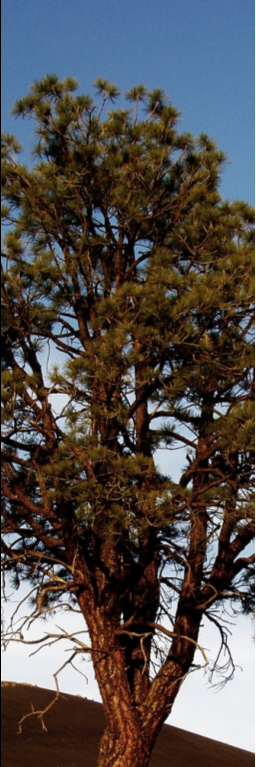
\includegraphics[width=2.3 cm,height=9.7 cm]{figs/Selection_008}}
\end{picture}
\frametitle{Outline}
\scriptsize{
\tableofcontents[currentsection,
    sectionstyle=show/show,
    subsectionstyle=show/show/hide]}
\end{frame}

\section{History}

\subsection{Administration}
\begin{frame}
\frametitle{Administration \\ {\large Class Rules}}
\begin{itemize}
  \item {\bf cheating}: Warning, then marks for one question deducted, then 0.
  \item {\bf Not putting pens down on exam finish}: Marks for one question deducted.
  \item {\bf Sleepy}: Get up, go drink a glass of water.
  \item {\bf Bathroom} Any time
  \item {\bf Extra help}: Bring your notebook, show your effort, ask specific questions.
  \item {\bf Talk to fellow students}: Sure, just don't disturb the class.
  \item {\bf Exam make-ups}: None, unless you missed because of an emergency. You will get an average
of your own averages and class-average.
\end{itemize}
\end{frame}

\begin{frame}
\frametitle{Administration \\ {\large Contact}}
\begin{itemize}
  \item E-mail:  \href{mailto:qaziejazurrehman@gmail.com}{qaziejazurrehman@gmail.com}
  \item Office hours: After 11:00 am
\end{itemize}
\end{frame}

\subsection{Introduction}
\begin{frame}
\frametitle{Introduction}
\framesubtitle{A Brief Introduction}
\begin{figure}[!tbp]
\centering
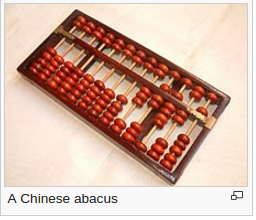
\includegraphics[scale = 0.55]{figs/Selection_002.png}
\end{figure}
\begin{itemize}
\item[\ding{45}] The only mechanical device that existed for numerical computation at the beginning of human history was the abacus, invented in Sumeria circa 2500 BC
\item[\ding{45}] And is still widely used by merchants, traders and clerks in Asia, Africa, and elsewhere
\end{itemize}
\end{frame}

\begin{frame}
\frametitle{Introduction}
\framesubtitle{Antikythera mechanism}
\begin{figure}[!tbp]
\centering
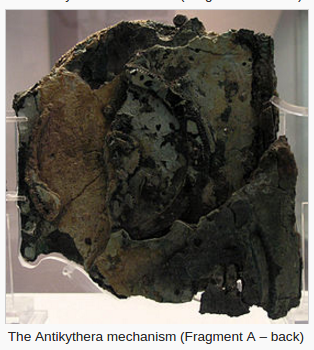
\includegraphics[scale = 0.35]{figs/bn.png}
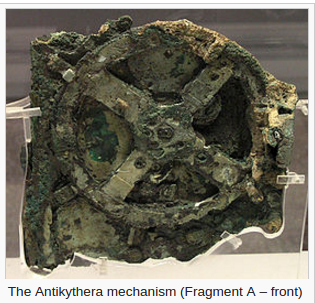
\includegraphics[scale = 0.4]{figs/bm.png}
\end{figure}
\small{
\begin{itemize}
\item[\ding{45}] The Antikythera mechanism, some time around 100 BC in ancient Greece, is the first known analog computer (mechanical calculator)
\item[\ding{45}] Designed to predict astronomical positions and eclipses for calendrical and astrological purposes as well as the Olympiads, the cycles of the ancient Olympic Games
\end{itemize}}
\end{frame}


\begin{frame}
\frametitle{Introduction}
\framesubtitle{$Badi'al-Zaman \ Ab\bar{u} \ al-'Izz \ Ism\bar{a}'\bar{i}l \newline ibn al-Raz\bar{a}z al-Jazar\bar{i}$}
\begin{itemize}
\item[\ding{45}] The Kurdish medieval scientist Al-Jazari built programmable automata\footnote{Same Idea as in Movie Automata (2014)} in 1206 AD.
\item Born: 1136 CE
\item Era: Islamic GOlden Age
\item Died: 1206 CE
\end{itemize}
\end{frame}

\begin{frame}
\frametitle{Introduction}
\framesubtitle{Johann Bernoulli \footnote{\url{http://en.wikipedia.org/wiki/Johann Bernoulli}}}
\begin{figure}[!tbp]
\centering
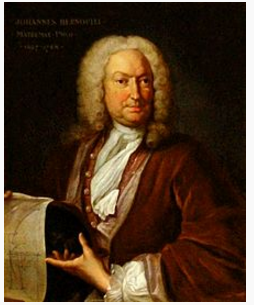
\includegraphics[scale = 0.35]{figs/Selection_0122.png}
\end{figure}
\begin{itemize}
\item 1667: Born in Switzerland, son of an apothecary
(in medical profession)
\item 1738: His son, Daniel Bernoulli published
\textit{Bernoulli's} principle
\item Students include his son Daniel, \em{\sc{Euler}}, L'Hopital
\item 1748: Death
\end{itemize}
\end{frame}

\begin{frame}
\frametitle{Introduction}
\framesubtitle{Leonhard Euler \tiny{\footnote{\url{ http://en.wikipedia.org/wiki/Leonhard Euler}}}}
\begin{figure}[!tbp]
\centering
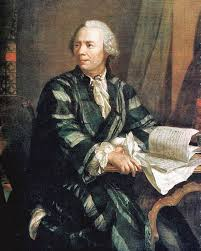
\includegraphics[scale = 0.35]{figs/download.jpg}
\end{figure}
\small{
\begin{itemize}
\item 1707: Born in Switzerland, son of a pastor
\item Among several other things, developed Euler's
identity, $e^{j\omega} = cos(\omega) + jsin(\omega)$
\item Also developed marvelous polyhedral fromula, nowadays written as "$v\ - \ e \ +\ f \ = \ 2$".
\item Friend of his doctoral advisor’s son, Daniel
Bernoulli, who developed Bernoulli’s principle
\item 1783: Death
\end{itemize}}
\end{frame}


\begin{frame}
\frametitle{Introduction}
\framesubtitle{Pierre-Simon Laplace \tiny{\footnote{http://en.wikipedia.org/wiki/Pierre-Simon Laplace}}}
\begin{figure}[!tbp]
\centering
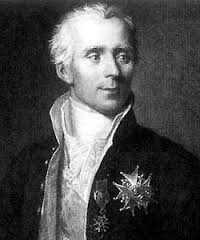
\includegraphics[scale = 0.35]{figs/zxc.jpg}
\end{figure}
\small{
\begin{itemize}
\item 1749: Born in France, son of a laborer
\item 1770-death: Worked on probability, celestial
mechanics, heat theory
\item 1785: Examiner, examined and passed Napoleon in
exam
\item 1790: Paris Academy of Sciences, worked with
Lavoisier, Coulomb
\item 1827: Died
\end{itemize}}
\end{frame}

\begin{frame}
\frametitle{Introduction}
\framesubtitle{Joseph Fourier \tiny{\footnote {\url{http://en.wikipedia.org/wiki/Joseph Fourier}}}}
\begin{figure}[!tbp]
\centering
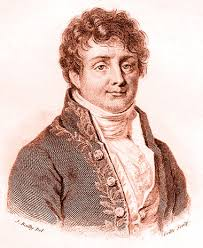
\includegraphics[scale = 0.35]{figs/cvb.jpg}
\end{figure}
\small{
\begin{itemize}
\item 1768: Born in France, son of a tailor
\item 1789-1799: Promoted the French Revolution
\item 1798: Went with Napoleon to Egypt and made
governor of Lower Egypt
\item 1822: Showed that representing a function by a
trigonometric series greatly simplifies the study of
heat propagation
\item1830: Fell from stairs and died shortly afterward
\end{itemize}}
\end{frame}



\begin{frame}
\frametitle{Introduction}
\framesubtitle{Charles Babbage}
\begin{figure}[!tbp]
\centering
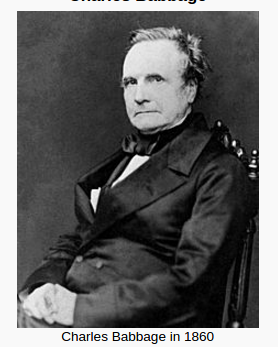
\includegraphics[scale = 0.35]{figs/Selection_006.png}
\end{figure}
\small{
\begin{itemize}
\item[\ding{45}]  Babbage is credited with inventing the first mechanical computer that eventually led to more complex designs.
\item Born: 26 December 1791 London, England   
\item Considered by some to be a "father of the computer"
\item Died: 18 October 1871 (aged 79) Marylebone, London, England
\end{itemize}}
\end{frame}

\begin{frame}
\frametitle{Introduction}
\framesubtitle{John Vincent Atanasoff (1903-1995)}
\begin{figure}[!tbp]
\centering
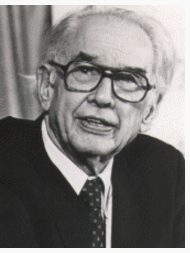
\includegraphics[scale = 0.5]{figs/Selection_01a2.png}
\caption[]{Atanasoff, in the 1990s.}
\end{figure}
Built first digital computer in the 1930s.
\end{frame}

\begin{frame}
\frametitle{Introduction}
\framesubtitle{Howard Hathaway Aiken (1901-1980)}
\begin{figure}[!tbp]
\centering
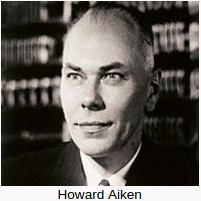
\includegraphics[scale = 0.5]{figs/Selection_01b2.png}
\end{figure}
\begin{itemize}
\item Built Mark I, during 1939-1944
\item Presented to public in 1944
\item Reaction was great
\begin{itemize}
\item Although Mark I meant a great deal for the development in
computer science, it's not recognised greatly today.
\item The reason for this is the fact that Mark I (and also Mark
II) was not electronic - it was electromagnetical
\end{itemize}
\end{itemize}
\end{frame}

\begin{frame}
\frametitle{Introduction}
\framesubtitle{J. Presper Eckert (1919-1995) and \\ Mauchly (1907-1980)}
\begin{figure}[!tbp]
\centering
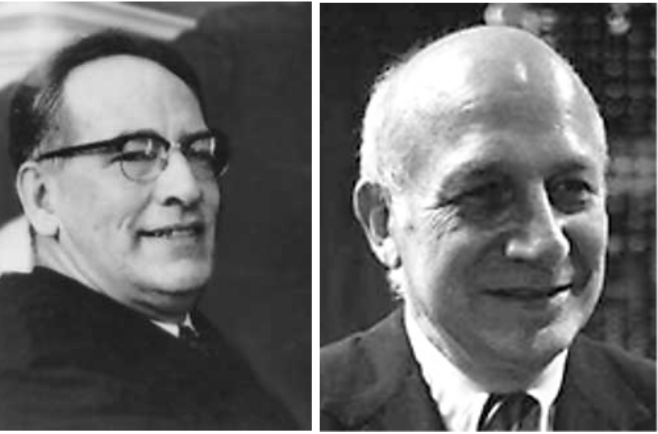
\includegraphics[scale = 0.31]{figs/Selection_01c2.png}
\end{figure}
Built ENIAC (Electronic Numerical Integrator and Computer), the first
electronic general-purpose computer during 1943-1945 at a cost of
\$468,000.
\end{frame}


\begin{frame}
\frametitle{Introduction}
\framesubtitle{Alan Mathison Turing\footnote{The Imitation Game: A 2014 Movie biographied on turing}}
\begin{figure}[!tbp]
\centering
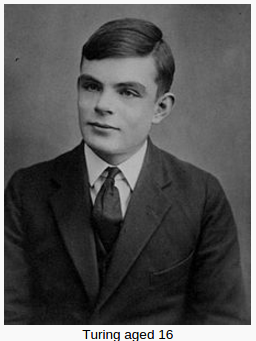
\includegraphics[scale = 0.35]{figs/alan.png}
\end{figure}
\begin{itemize}
\item {\bf Born}: 23 June 1912
\item Turing is widely considered to be the father of theoretical computer science and artificial intelligence
\item Famous for Breaking Enigma Machine Code
\item {\bf Died}: 7 June 1954 (aged 41)
\end{itemize}
\end{frame}

\begin{frame}
\frametitle{Turing Machine}
\begin{tikzpicture}
\tikzstyle{every path}=[very thick]

\edef\sizetape{0.7cm}
\tikzstyle{tmtape}=[draw,minimum size=\sizetape]
\tikzstyle{tmhead}=[arrow box,draw,minimum size=.5cm,arrow box
arrows={east:.25cm, west:0.25cm}]

%% Draw TM tape
\begin{scope}[start chain=1 going right,node distance=-0.15mm]
    \node [on chain=1,tmtape,draw=none] {$\ldots$};
    \node [on chain=1,tmtape] {};
    \node [on chain=1,tmtape] (input) {b};
    \node [on chain=1,tmtape] {b};
    \node [on chain=1,tmtape] {a};
    \node [on chain=1,tmtape] {a};
    \node [on chain=1,tmtape] {a};
    \node [on chain=1,tmtape] {a};
    \node [on chain=1,tmtape] {};
    \node [on chain=1,tmtape,draw=none] {$\ldots$};
    \node [on chain=1] {\textbf{\scriptsize{Input/Output Tape}}};
\end{scope}
%% Draw TM Finite Control
\begin{scope}
[shift={(3cm,-5cm)},start chain=circle placed {at=(-\tikzchaincount*60:1.5)}]
\foreach \i in {q_0,q_1,q_2,q_3,\ddots,q_n}
	\node [on chain] {$\i$};

% Arrow to current state
\node (center) {};
\draw[->] (center) -- (circle-2);

\node[rounded corners,draw=black,thick,fit=(circle-1) (circle-2) (circle-3) 
      (circle-4) (circle-5) (circle-6),
			label=below:\textbf{Finite Control}] (fsbox)
		{};
\end{scope}

%% Draw TM head below (input) tape cell
\node [tmhead,yshift=-.3cm] at (input.south) (head) {$q_1$};

%% Link Finite Control with Head
\path[->,draw] (fsbox.north) .. controls (4.5,-1) and (0,-2) .. node[right] 
			(headlinetext)
 			{} 
			(head.south);
\node[xshift=3cm] at (headlinetext)  
			{\begin{tabular}{c} 
				\textbf{Reading and Writing Head} \\  
				\textbf{(moves in both directions)} 
			 \end{tabular}};

\end{tikzpicture}
\end{frame}

\begin{frame}
\frametitle{History \\ {\large FORTRAN}}
\begin{figure}[!tbp]
\centering
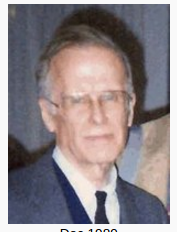
\includegraphics[scale = 0.35]{figs/Selection_007.png}
\end{figure}
\begin{itemize}
\item Inventor: John Backus
\item[\ding{45}]  FORTRAN, derived from Formula Translating System
\item It is a general-purpose, imperative programming language that is especially suited to numeric computation and scientific computing. Originally developed by IBM
\item First Appeared: 1957; 59 years ago
\end{itemize}
\end{frame}

\begin{frame}
\frametitle{History \\ {\large C++}}
\begin{figure}[!tbp]
\centering
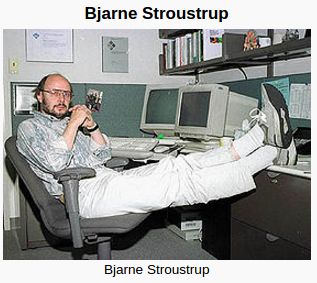
\includegraphics[scale = 0.35]{figs/cpr.png}
\end{figure}
\scriptsize{
\begin{itemize}
\item Inventor: Bjarne Stroustrup (at Bell Labs)
\item It is a general-purpose programming language. It has imperative, object-oriented and generic programming features, while also providing facilities for low-level memory manipulation
\item C++ is standardized by the International Organization for Standardization (ISO)
\item First Appeared: 1983; 33 years ago
\end{itemize}}
\end{frame}

\begin{frame}[shrink]%allowframebreaks]
\frametitle{Excellence of Human}
\framesubtitle{Equations: Changed The World}
\footnotesize{
 \resizebox{\linewidth}{!}{
%\begin{center}
\begin{tabular}{p{3.5cm} p{4.5cm} p{3cm}}
\\ \\ 
 \multicolumn{3}{c}{\textcolor{olive}{17 Equations That Changed The World}} \\ \\
 Pythagora.s Theorem&$a^2+b^2=c^2$&Pythagoras,530 BC\\
 Logarithms&$logxy=logx+logy$& John Napier, 1610\\
 Calculus &$\frac{df}{dt}=\lim_{h \to 0}\frac{f(t+h)-f(t)}{h}$& Newton, 1668\\
Law of Gravity   &$F=G\frac{m_1m_2}{r^2}$& Newton, 1687\\
Complex Identity&$i^2=-1$& Euler, 1750\\
Polyhedra Formula&$V-E+F=2$& Euler, 1751\\
Normal Distribution&$\phi(x)=\frac{1}{\sqrt{2\pi\rho}}e^\frac{(x-\mu)^2}{2\rho^2}$& C.F. Gauss, 1810\\
Wave Equation&$\frac{\partial^2u}{\partial t^2}=c^2\frac{\partial^2u}{\partial x^2}$& J. d'Almbert,1746\\
Fourier Transform&$f(\omega)=\int_{-\infty}^\infty f(x)e^{-2\pi ix\omega}dx$& J. Fourier, 1822\\
Navier-Stokes Equation&$\rho(\frac{\partial v}{\partial t}+v.\nabla v)=-\nabla p+\nabla .T+f$& C. Navier, G. Stokes, 1845\\
Maxwell's Equations& {\tiny{\begin{tabular}{c c}
$\nabla  E=\frac{\rho}{\epsilon 0}$ & $\nabla .H=0$ \\ 
$\nabla \times E=-\frac{1}{c}\frac{\partial H}{\partial t}$ & $\nabla \times H=\frac{1}{c}\frac{\partial E}{\partial t}$
\end{tabular}}}& J.C. Maxwell, 1865\\
Second Law of Thermosynamics &$dS\ge0$ & L. Boltzmann, 1874\\
Relativity & $E=mc^2$&Einstein, 1905\\
Schrodinger's Equation &$i\hslash\frac{\partial}{\partial t}\Psi=H\Psi$&E. Schrodinger, 1927\\
Information Theory &$H=-\sum p(x)logp(x)$&C. Shannon, 1949 \\
Chaos Theory &$x_{t+1}=kx_t(1-x_t)$& Robert May,1975\\
Black-Scholes\\ Equation&$\frac{1}{2}\sigma^2S^2\frac{\partial^2V}{\partial S^2}+rS\frac{\partial V}{\partial S}+\frac{\partial V}{\partial t}-rV=0$&F. Black, M. Scholes, 1990\\
\end{tabular}}}
%\end{center}}}
\end{frame}









\begin{frame}
\frametitle{Introduction \\ {\large Modern programming}}
Whatever the approach to development may be, the final program must satisfy some fundamental properties. The following properties are among the most important
\begin{itemize}
\item[\ding{90}] Reliability
\item[\ding{90}] Robustness
\item[\ding{90}] Usability
\item[\ding{90}] Portability
\item[\ding{90}] Maintainability
\item[\ding{90}] Efficiency/performance
\end{itemize}
\end{frame}

\begin{frame}
\frametitle{History \\ {\large 4GL}}
Some fourth generation programming language
\begin{itemize}
\item Matlab/Simulink
\item LabVIEW
\item Python
\item Wolfram
\item Unix Shell
\end{itemize}
\end{frame}

\subsection{Matlab}
\begin{frame}
\frametitle{Introduction\\ {\large Matlab}}
\begin{figure}[!tbp]
\centering
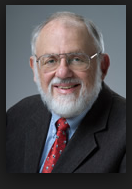
\includegraphics[scale = 0.5]{figs/matl.png}
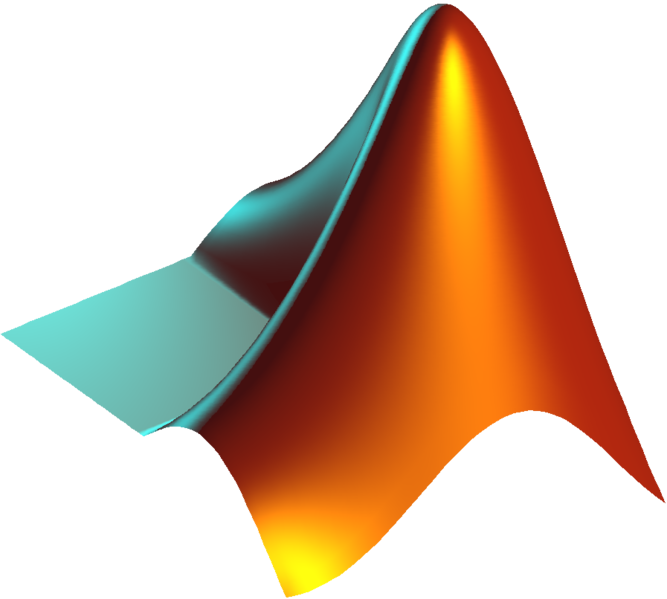
\includegraphics[scale = 0.08]{figs/Selection_035.png}
\end{figure}
\small{
\begin{itemize}
\item Initial Release: 1984; 32 years ago
\item MATLAB is a multi-paradigm numerical computing environment and fourth-generation programming language
\item Widely Used for Academic, Research \& Development
\item Cross-Platform Software
\item Latest Stable Release: Matlab R2015b
\end{itemize}}
\end{frame}

\subsection{LabVIEW}
\begin{frame}
\frametitle{Introduction\\ {\large LabVIEW}}
\begin{figure}[!tbp]
\centering

\includegraphics[scale = 0.5]{figs/fg.png}
\end{figure}
\begin{itemize}
\item Initial Release: 1983; 33 years ago
\item LabVIEW (short for Laboratory Virtual Instrument Engineering Workbench) is a system-design platform and development environment for a visual programming language from National Instruments
\item The graphical language is named "G" used by LabVIEW
\item Cross-Platform Software
\item Latest Stable Release: 2015/ August 2015
\end{itemize}
\end{frame}







%%%%%%%%%%%%%%%%%%%%%%%%
\subsection{Basic Math}
\begin{frame}
\frametitle{Calculus \\ {\large Integration by parts}}
\begin{figure}[!tbp]
\centering
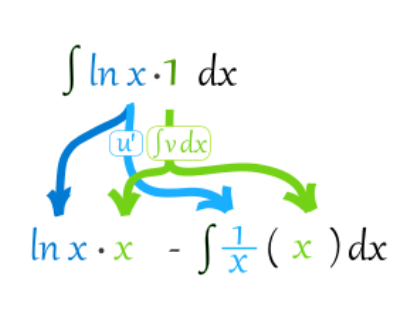
\includegraphics[scale = 0.35]{figs/ab.png}
\footnote{\href{http://www.mathsisfun.com/calculus/integration-by-parts.html}{\beamergotobutton{Link}}}
\end{figure}
\end{frame}
\begin{frame}
\frametitle{Linear Algebra \\ {\large Partial fraction expansion}}
\begin{figure}[!tbp]
\centering
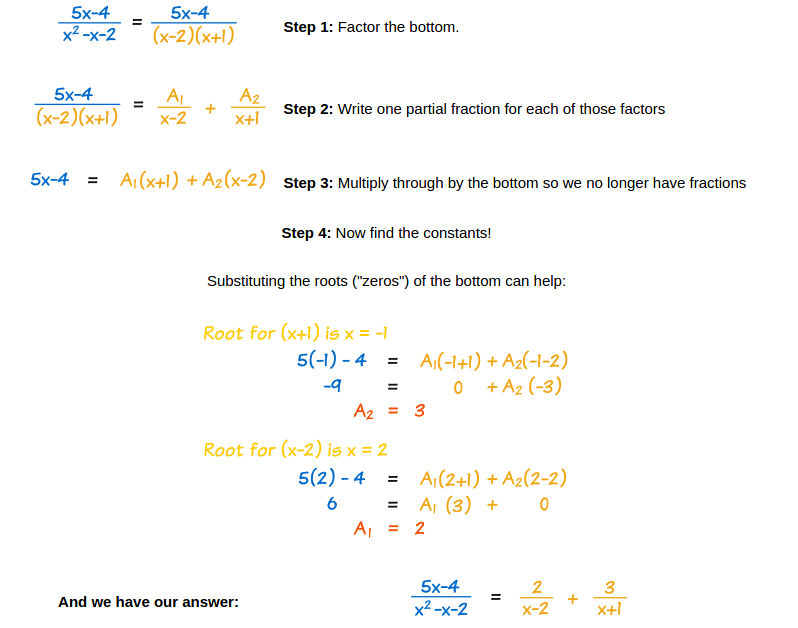
\includegraphics[scale = 0.3]{figs/Selection_012.png}
\footnote{\href{http://www.mathsisfun.com/calculus/integration-by-parts.html}{\beamergotobutton{Link}}}
\end{figure}
\end{frame}
\begin{frame}
\frametitle{Linear Algebra \\ {\large Determinants}}
Here's an easy illustration that shows why the \textcolor{blue}{determinant} of a matrix with \textcolor{blue}{linear dependent} rows is 0

$$M=\begin{bmatrix}
    a       & b \\
    2a     &2b \\
\end{bmatrix}$$
$$\Rightarrow |M|=a(2b) - 2b(a)=0$$  \\
Let's look at a 3x3 example.
\end{frame}

\begin{frame}
\frametitle{Linear Algebra \\ {\large Determinants}}
$M=\begin{bmatrix}
    a       & b  &c\\
    2a     &2b &c\\
    d       &e   &f\\
\end{bmatrix}$ \\
$\Rightarrow |M|=a(2bf-2ce) - b(2af-2cd)+c(2ae-2bd)=0$ \\
Let's change the order of rows \\
$M=\begin{bmatrix}
 d       &e   &f\\   
 a       & b  &c\\
    2a     &2b &c\\
\end{bmatrix}$ \\
$\Rightarrow |M|=d(2bc - 2bc) - e(2ac - 2ac) + f (2ab - 2ab)=0$
Let's change the order of rows again\\
$M=\begin{bmatrix}
 d       &e   &f\\ 
 2a     &2b &c\\  
 a       & b  &c\\
\end{bmatrix}$ \\
$\Rightarrow |M|=a(2ce - 2bf ) - b(2dc - 2af ) + c(2db - 2ae)=0$ \\
In other words, if we have dependent rows, then the determinant of the
matrix is 0
\end{frame}
  
\begin{frame}
\frametitle{Linear Algebra \\ {\large Adjoint of matrix}}
\begin{figure}[!tbp]
\centering
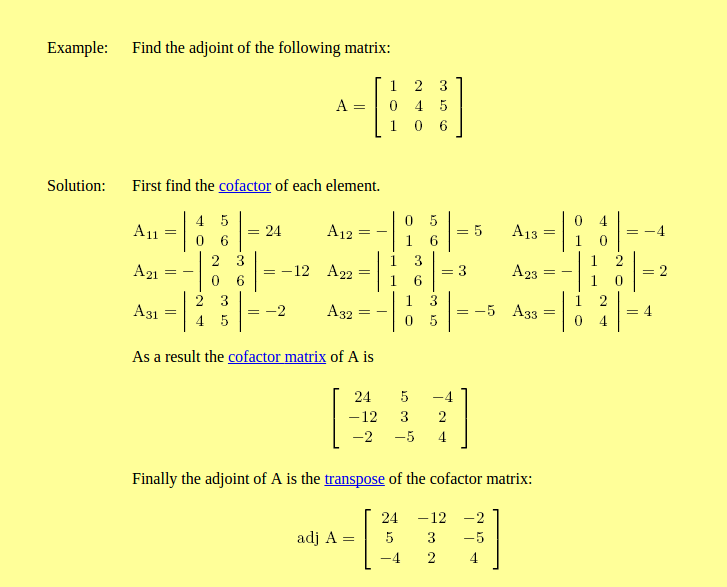
\includegraphics[scale = 0.35]{figs/Selection_013.png}
\footnote{\href{http://www.mathwords.com/a/adjoint.htm}{\beamergotobutton{Link}}}
\end{figure}
\end{frame}

\begin{frame}
\frametitle{Linear Algebra \\ {\large Inverse of matrix}}
\begin{center}
$A^{-1}=\frac{1}{|A|}$(Adjoint of A)
\end{center}
\end{frame}

\begin{frame}
\frametitle{Laplace Transform \\ {\large Plot of simple first order equation}} 
Let $H(s) = \frac{1}{s+10}$,We've plotted the magnitude of H(s) below, i.e., $\vert H(s) \vert$. Other
possible 3D plots are $\angle$ H(s), Re(H(s)) and Im(H(s)) respectively. Notice that $|H(s)|$ goes to $\infty$
at the pole s = -10.
\begin{figure}[!tbp]
\centering
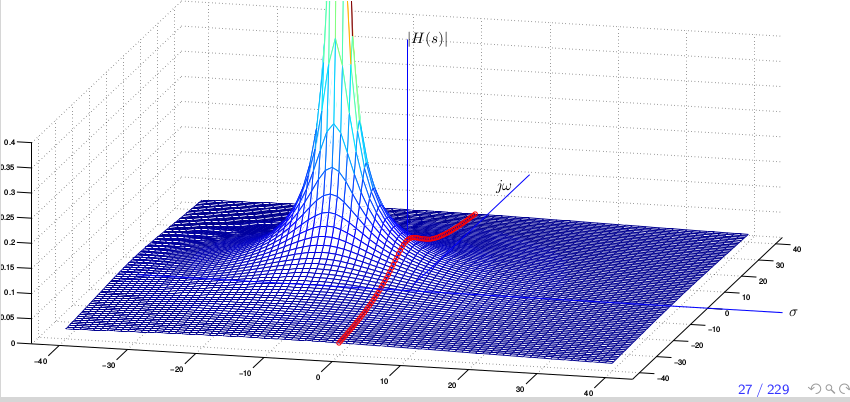
\includegraphics[scale = 0.4]{figs/Selection_016.png}
\end{figure}
\end{frame}


\begin{frame}
\frametitle{Laplace Transform}
\framesubtitle{3-D code for Transfer functions \attachfile{code/qazie.m}}

\begin{tcolorbox}[title=  ,width=9.85 cm]
\lstinputlisting{code/qazialpha.m}
\end{tcolorbox}
\end{frame}

\begin{frame}
\frametitle{Parabolic Graph}
\pagestyle{empty}
\begin{tikzpicture}[scale=1.8]
  \shade[top color=blue,bottom color=gray!50] 
      (0,0) parabola (1.5,2.25) |- (0,0);
  \draw (1.07cm,2pt) node[above] 
      {\scriptsize $\displaystyle\int_0^{3/2} \!\!x^2\mathrm{d}x$};

  \draw[style=help lines] (0,0) grid (3.9,3.9)
       [step=0.25cm]      (1,2) grid +(1,1);

  \draw[->] (-0.2,0) -- (4,0) node[right] {$x$};
  \draw[->] (0,-0.2) -- (0,4) node[above] {$f(x)$};

  \foreach \x/\xtext in {1/1, 1.5/1\frac{1}{2}, 2/2, 3/3}
    \draw[shift={(\x,0)}] (0pt,2pt) -- (0pt,-2pt) node[below] {$\xtext$};

  \foreach \y/\ytext in {1/1, 2/2, 2.25/2\frac{1}{4}, 3/3}
    \draw[shift={(0,\y)}] (2pt,0pt) -- (-2pt,0pt) node[left] {$\ytext$};

  \draw (-.5,.25) parabola bend (0,0) (2,4) node[below right] {$x^2$};
\end{tikzpicture}
\end{frame}



\begin{frame}
\frametitle{Polar and cartesian coordinates}
\small{
\pagestyle{empty}
\begin{tikzpicture}[scale=1.5,cap=round]
  % Local definitions
  \def\costhirty{0.8660256}

  % Colors
  \colorlet{anglecolor}{green!50!black}
  \colorlet{sincolor}{red}
  \colorlet{tancolor}{orange!80!black}
  \colorlet{coscolor}{blue}

  % Styles
  \tikzstyle{axes}=[]
  \tikzstyle{important line}=[very thick]
  \tikzstyle{information text}=[rounded corners,fill=red!10,inner sep=1ex]

  % The graphic
  \draw[style=help lines,step=0.5cm] (-1.4,-1.4) grid (1.4,1.4);

  \draw (0,0) circle (1cm);

  \begin{scope}[style=axes]
    \draw[->] (-1.5,0) -- (1.5,0) node[right] {$x$};
    \draw[->] (0,-1.5) -- (0,1.5) node[above] {$y$};

    \foreach \x/\xtext in {-1, -.5/-\frac{1}{2}, 1}
      \draw[xshift=\x cm] (0pt,1pt) -- (0pt,-1pt) node[below,fill=white]
            {$\xtext$};

    \foreach \y/\ytext in {-1, -.5/-\frac{1}{2}, .5/\frac{1}{2}, 1}
      \draw[yshift=\y cm] (1pt,0pt) -- (-1pt,0pt) node[left,fill=white]
            {$\ytext$};
  \end{scope}

  \filldraw[fill=green!20,draw=anglecolor] (0,0) -- (3mm,0pt) arc(0:30:3mm);
  \draw (15:2mm) node[anglecolor] {$\alpha$};

  \draw[style=important line,sincolor]
    (30:1cm) -- node[left=1pt,fill=white] {$\sin \alpha$} +(0,-.5);

  \draw[style=important line,coscolor]
    (0,0) -- node[below=2pt,fill=white] {$\cos \alpha$} (\costhirty,0);

  \draw[style=important line,tancolor] (1,0) --
    node [right=1pt,fill=white]
    {
      $\displaystyle \tan \alpha \color{black}=
      \frac{{\color{sincolor}\sin \alpha}}{\color{coscolor}\cos \alpha}$
    } (intersection of 0,0--30:1cm and 1,0--1,1) coordinate (t);

  \draw (0,0) -- (t);

  \draw[xshift=1.1cm] node [right,text width=6cm,style=information text]
    {
      The {\color{anglecolor} angle $\alpha$} is $30^\circ$ in the
      example ($\pi/6$ in radians). The {\color{sincolor}sine of
        $\alpha$}, which is the height of the red line, is
      \[
      {\color{sincolor} \sin \alpha} = 1/2.
      \]
      By the Theorem of Pythagoras we have ${\color{coscolor}\cos^2 \alpha} +
      {\color{sincolor}\sin^2\alpha} =1$. Thus the length of the blue
      line, which is the {\color{coscolor}cosine of $\alpha$}, must be
      \[
      {\color{coscolor}\cos\alpha} = \sqrt{1 - 1/4} = \textstyle
      \frac{1}{2} \sqrt 3.
      \]%
      This shows that {\color{tancolor}$\tan \alpha$}, which is the
      height of the orange line, is
      \[
      {\color{tancolor}\tan\alpha} = \frac{{\color{sincolor}\sin
          \alpha}}{\color{coscolor}\cos \alpha} = 1/\sqrt 3.
      \]%
    };
\end{tikzpicture}
}
\end{frame}
%%%%%%%%%%%%%%%%%%%%
\begin{frame}
\frametitle{Coordinate Transformation}
\begin{figure}[t]
\centering
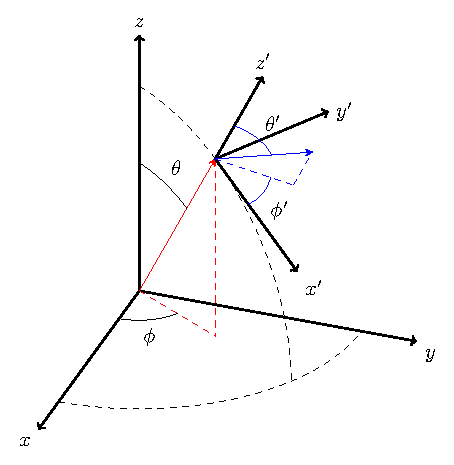
\includegraphics[scale=0.78]{spherical/b.pdf}
\caption{3-D plot Illustration}
\end{figure}
\end{frame}


\begin{frame}
\frametitle{Spherical and cartesian grids}
\begin{figure}[t]
\centering
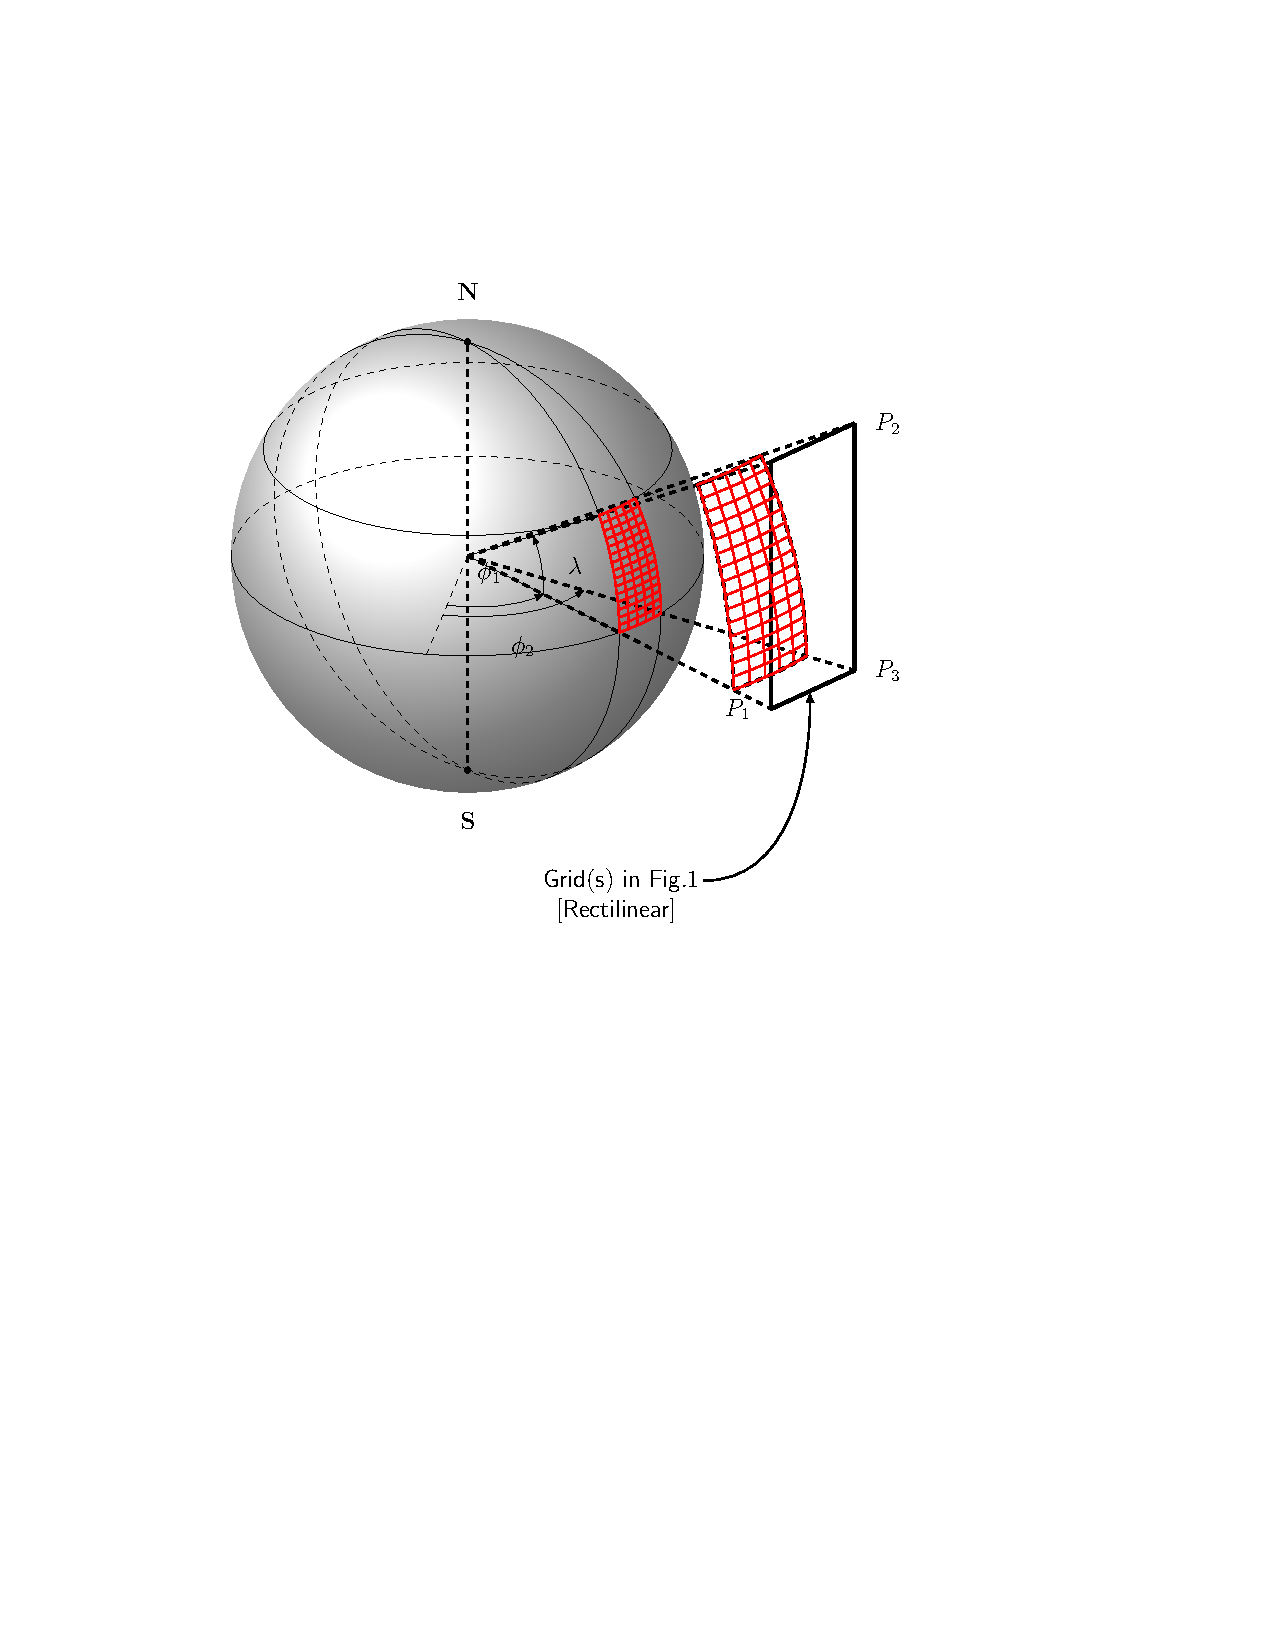
\includegraphics[scale=0.48]{spherical/a.pdf}
\end{figure}
\end{frame}



\begin{frame}
\frametitle{Differential Equations}
\small{
\begin{tikzpicture}
\node [mybox1] (box){%
    \begin{minipage}{0.93\textwidth}
        To calculate the horizonal position the kinematic differential
        equations are needed:
        \begin{align}
            \dot{n} &= u\cos\psi -v\sin\psi \\
            \dot{e} &= u\sin\psi + v\cos\psi
        \end{align}
        For small angles the following approximation can be used:
        \begin{align}
            \dot{n} &= u -v\delta_\psi \\
            \dot{e} &= u\delta_\psi + v
        \end{align}
    \end{minipage}
};
\node[fancytitle1, right=10pt] at (box.north west) {First order Differential Equations};
\node[fancytitle1, rounded corners] at (box.east) {$\clubsuit$};
\end{tikzpicture}%
}%
%
\end{frame}
%\hyperlink{contents}{\beamergotobutton{Back to immediate slide}}


\section{Modeling}

\subsection{Electrical}
\begin{frame}
\frametitle{Modeling\\ {\large RLC Circuit}} 
\begin{figure}[!t]
\centering
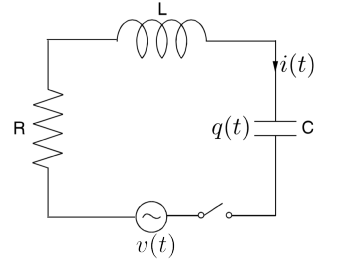
\includegraphics[scale = 0.35]{figs/Selection_020.png}
\end{figure}
\begin{align}
L \frac{di(t)}{dt}+Ri(t)+\frac{1}{C}q(t)=v(t) \\
 i(t)=\frac{dq(t)}{dt}
\end{align} 
\begin{eqnarray*}
\Rightarrow L\frac{d^2q(t)}{dt^2}+R\frac{dq(t)}{dt}+\frac{1}{C}q(t)=v(t) \\
\Rightarrow L\ddot{q}(t)+R\dot{q}(t)+\frac{1}{C}q(t)=\textcolor{mygreen}{v(t)}
\end{eqnarray*}
\end{frame}





\begin{frame}
\frametitle{Modeling\\ {\large C parallel with RL circuit}} 
\begin{figure}[!t]
\centering
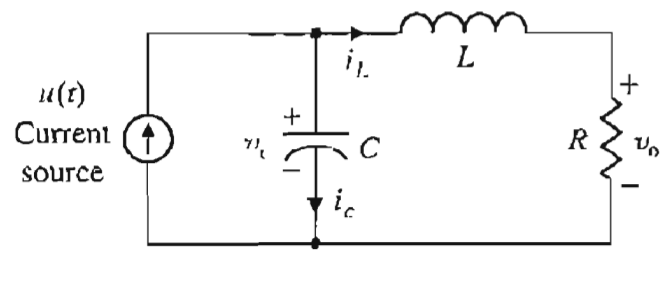
\includegraphics[scale = 0.25]{figs/Selection_021.png}
\end{figure}
\begin{eqnarray*}
i_C=-\textcolor{blue}{i_L}+u(t) \\
\Rightarrow C\frac{d\textcolor{red}{v_C}}{dt}=-\textcolor{blue}{i_L}+u(t) \\
\Rightarrow \frac{d\textcolor{red}{v_C}}{dt}=-\frac{1}{C}\textcolor{blue}{i_L}+\frac{1}{C}u(t)
\\  \newline \newline
V_C=V_L+\textcolor{blue}{i_L}R 
\\ = L\frac{d\textcolor{blue}{i_L}}{dt}+i_LR
\end{eqnarray*}
solve for $\frac{d\textcolor{blue}{i_L}}{dt}$
\end{frame}



\subsection{Mechanical}

\begin{frame}
\frametitle{Modeling\\ {\large Constant acceleration model}} 
\tiny{
$$\ddot{s}(t)=a$$
\noindent\makebox[\linewidth]{\rule{10 cm}{0.1pt}}
\begin{align*}
\int_{t_0}^t \ddot{s}(\tau) \ d\tau=\int_{t_0}^t a \ d\tau \\
\textcolor{blue}{\dot{s}}(\tau)|^t_{t_0} = a \  \tau|^t_{t_0} \\
\textcolor{blue}{\dot{s}}(t) - \textcolor{blue}{\dot{s}}(t_0) = at-a\textcolor{red}{t_0}
\end{align*}
\noindent\makebox[\linewidth]{\rule{10 cm}{0.1pt}}
\begin{align*}
\int_{t_0}^t \textcolor{blue}{\dot{s}}(\tau)d\tau - \int_{t_0}^t \textcolor{blue}{\dot{s}}(t_0) d \tau = \int_{t_0}^t a\tau d\tau - \int_{t_0}^t a\textcolor{red}{t_0}d\tau \\
\textcolor{red}{s}(\tau)|^t_{t_0}-\textcolor{blue}{\dot{s}}(t_0)\tau|^t_{t_0}  = \frac{1}{2}a \  \tau^2|^t_{t_0}-at_0\tau|^t_{t_0} \\
\textcolor{red}{s}(t)-\textcolor{red}{s}(t_0)-\textcolor{blue}{\dot s}(t_0)t+\textcolor{blue}{\dot s}(t_0)\textcolor{red}{t_0}=\frac{1}{2}\textcolor{mygreen}{a}t^2-\frac{1}{2}\textcolor{mygreen}{a}\textcolor{red}{t_0}^2-\textcolor{mygreen}{a}\textcolor{red}{t_0}t+\textcolor{mygreen}{a}\textcolor{red}{t_0}^2
\end{align*}
\noindent\makebox[\linewidth]{\rule{10 cm}{0.1pt}}
let initial time $t_0 = 0$, initial distance $\textcolor{red}{s}(t_ 0) = 0$, and some initial velocity
$\textcolor{blue}{\dot s}(t_0) = \textcolor{blue}{v_i}$, to get the familiar equation,
$$\textcolor{red}{s}(t)=\textcolor{blue}{v_i}t+\frac{1}{2}at^2$$
If we take the derivative with respect to t, we get $\textcolor{blue}{v_f}= \textcolor{blue}{v_i} + at$
}
\end{frame}





\begin{frame}
\frametitle{Modeling\\ {\large DC Motor {\tiny cont..}}} 
\tiny{
\begin{columns}
    \begin{column}{0.9\textwidth}
\put(-5,210){$\textcolor{red}{v_b}=K_b \omega$} \put(-5,200){$ = K_b \dot{\theta} $ }
\put(25,200){
%\begin{tcolorbox}[colback=mygreen!5,colframe=mygreen!40!black,title=Time Domain]
\colorbox{pink}{\parbox{3.65 cm}{
\centering
Differential equations 
\begin{flushleft}
 \fbox{\begin{minipage}[t]{15em}
\begin{align*}
%\parbox{\textwidth}
\colorbox{cyan}{\hbox to 0.3 mm{L\hfill}} \frac{di}{dt}&+\colorbox{cyan}{\hbox to 0.3 mm{R\hfill}}i=\textcolor{red}{v}-\textcolor{red}{v_b} & \text{1} \\
\colorbox{yellow}{\hbox to 0.3 mm{J\hfill}}\ddot{\theta}&+\colorbox{yellow}{\hbox to 0.3 mm{b\hfill}}\dot{\theta}=\colorbox{  white}{\hbox to 2.2 mm{\textit{${K_m}$}\hfill}}\hspace{1 pt} i  & \text{2}
\end{align*}
\end{minipage}}
\end{flushleft}
%\colorbox{cyan}{\makebox[12em]{\strut\textcolor{black}{R:electrical resistance \ 1 ohm }}}
\colorbox{cyan}{\parbox{2.75 cm}{\color{black}R: electrical resistance \ 1 ohm \\ L: electrical inductance \ 0.5H }}
\colorbox{yellow}{\parbox{3.4 cm}{\color{black}J: moment of inertia \ 0.01 kg.$m^2$ \\ b: motor friction constant \ 0.1 N.m.s }}

\colorbox{white}{\parbox{3.4 cm}{\color{black}$K_b$: emf constant \ 0.01 V/rad/sec \\ Km: torque constant 0.01 N.m/Amp }}
\hyperlink{motor1}
\hfill}}
%\end{tcolorbox}
}\put(-10,140){\hyperlink{motor1}{\beamergotobutton{Lab 2}}}
\put(-10,260){
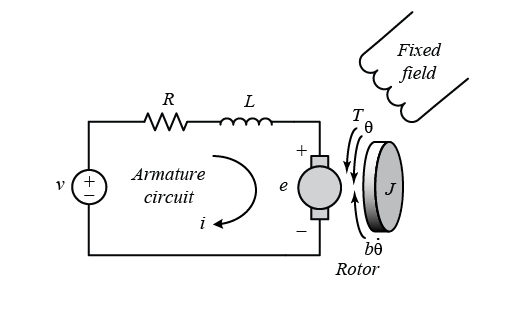
\includegraphics[scale = 0.3]{figs/Selection_022.png}
}
\end{column}
    \begin{column}{0.05\textwidth}
\end{column}    
\end{columns}
}
\label{motor}
\end{frame}

\subsection{Aerospace}



\begin{frame}
\frametitle{Modeling\\ {\large Pitch Control {\tiny cont..}}}
\begin{figure}[!tbp]
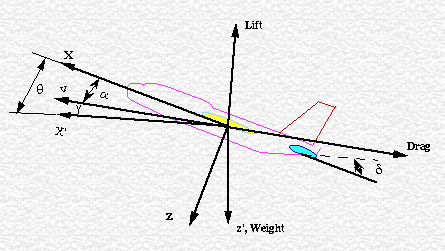
\includegraphics[scale = 0.35]{figs/Selection_041.png}
 \caption{Boeing}
\end{figure}
\small{
Assume that the aircraft is in steady-cruise at constant altitude and velocity; thus, the thrust and drag cancel out and the lift and weight balance out each other. Also, assume that change in pitch angle does not change the speed of an aircraft under any circumstance (unrealistic but simplifies the problem a bit). Under these assumptions, the longitudinal equations of motion of an aircraft can be written as:}
\end{frame}

\begin{frame}
\frametitle{Modeling\\ {\large Pitch Control {\tiny cont..}}}
\scriptsize{
\begin{align*}
\dot{\alpha}&=\mu\Omega\sigma[-(C_L+C_{D_0})\alpha+(1/ \mu -C_L)q-(C_wSin\gamma_e)\theta+C_L] \\ 
\dot{q}&=\mu\Omega/2i_n \Bigg[ [C_M-\eta(C_L+C_{D_0})]\alpha 
 + [C_M+\sigma C_M(1-\mu C_L)]q \\ +& (\eta C_Wsin\gamma_e)\delta_3) \Bigg] \ \text(1) \\
\dot{\theta}&=\Omega q
\end{align*}
Where: \\
 $\alpha$=Angle of attack,  
q=Pitch rate, 
$\theta$=Pitch angle, 
$\delta $=Elevator deflection angle,  
$\mu=\frac{\rho S\bar{c}}{4m}$,
$C_T$=Coefficient of thrust, $C_D$=Coefficient of Drag, $C_L$=Coefficient of lift, $C_W$=coefficient of weight, $C_M$=coefficient of pitch moment , $\gamma_e$ = Flight path angle
\begin{itemize}
\item[] $\rho$ = Density of air
\item[] S = Planform area of the wing 
\item[] $\bar{c}$ = Average chord length
\item[] m= Mass of aircraft
\end{itemize}
$\Omega=\frac{2U}{\bar{c}}$ \\
U =equilibrium flight speed, 
$\sigma =\frac{1}{1+\mu C_L}$, $i_n$=Normalized moment of inertia, $\eta=\mu \sigma C$ \ = constant nu
}
\end{frame}


\begin{frame}
\frametitle{Modeling\\ {\large Pitch Control {\tiny cont..}}}
Before finding transfer function and the state-space model, let's plug in some numerical values to simplify the modeling equations (1) shown in previous slide.
\begin{align*}
\dot{\alpha}&=-0.313\alpha+56.7q+0.232 \delta_e \\ 
\dot{q}&=-0.0139\alpha -0.426q + 0.0203 \delta_e \ \text(2) \\
\dot{\theta}&=56.7 q
\end{align*}
These values are taken from the data from one of the Boeing's commercial aircraft.
\end{frame}
%%%%%%%%%%%%%%%%%%%%%%%%%%%%%%
\section{Software}
\begin{frame}
\frametitle{Intro. to Matlab}
\begin{flushright}
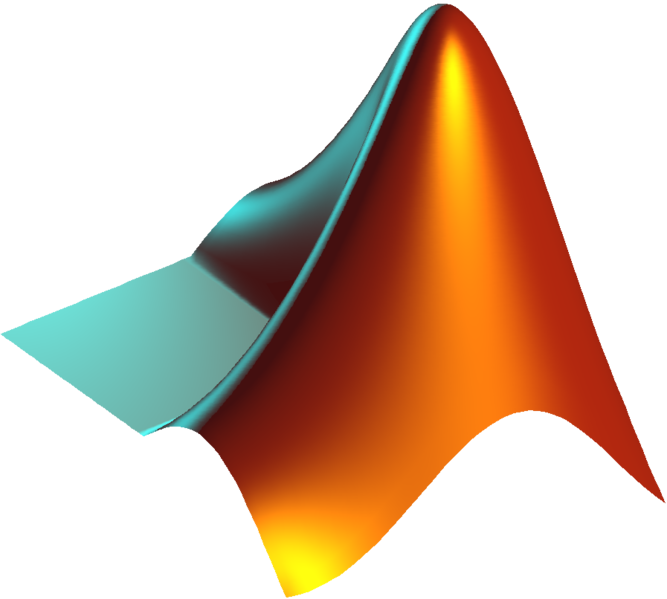
\includegraphics[scale = 0.08]{figs/Selection_035.png}
\end{flushright}
\begin{enumerate}
\item<1-> The name MATLAB stands for \textcolor{cyan}{MATrix LABoratory}. 
\item<2-> MATLAB was written originally to provide easy access to matrix software developed by the LINPACK (linear system package) and EISPACK (Eigen system package) projects.
\item<3-> MATLAB has a number of competitors. Commercial competitors include \textcolor{blue}{Mathematica}, \textcolor{blue}{ TK Solver}, \textcolor{blue}{Maple}, and  \textcolor{blue}{IDL}.
\item<4-> There are also free open source alternatives to MATLAB, in particular  \textcolor{red}{GNU Octave}, \textcolor{red}{Scilab}, \textcolor{red}{FreeMat}, \textcolor{red}{Julia}, and \textcolor{red}{Sage} which are intended to be mostly compatible with the MATLAB language.
\item<5-> MATLAB was first adopted by researchers and practitioners in control engineering.
\end{enumerate}
\end{frame}


\begin{frame}
\frametitle{Intro. to Simulink \\ {\large An essential part of Matlab}}
\begin{flushright}
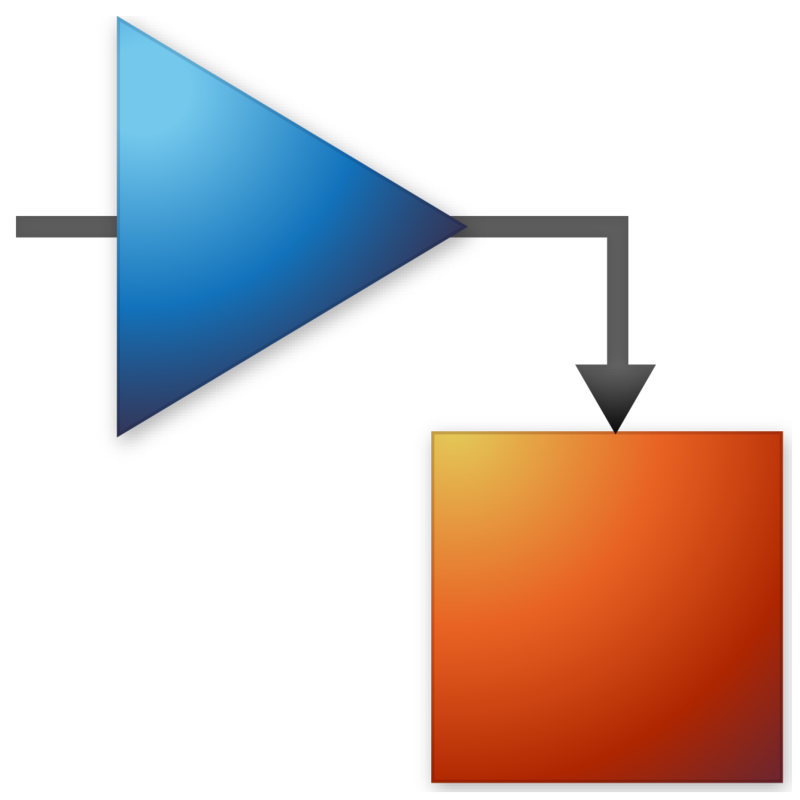
\includegraphics[scale = 0.05]{figs/Selection_036.png}
\end{flushright}
\begin{enumerate}
\item The name Simulink stands for Simulations and links
\item Old name was Simulab 
\item Simulink is widely used in automatic control and digital signal processing for multidomain simulation and Model-Based Design.
\end{enumerate}
\end{frame}

\begin{frame}
\frametitle{Intro. to Matlab}
\begin{flushright}
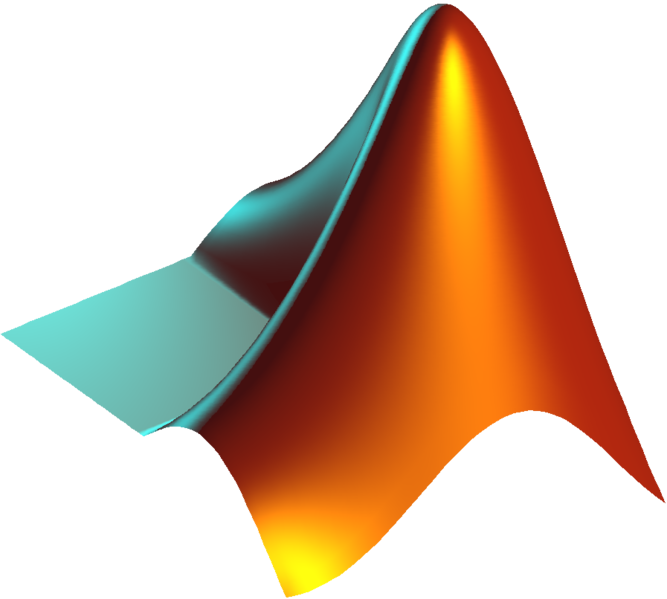
\includegraphics[scale = 0.08]{figs/Selection_035.png}
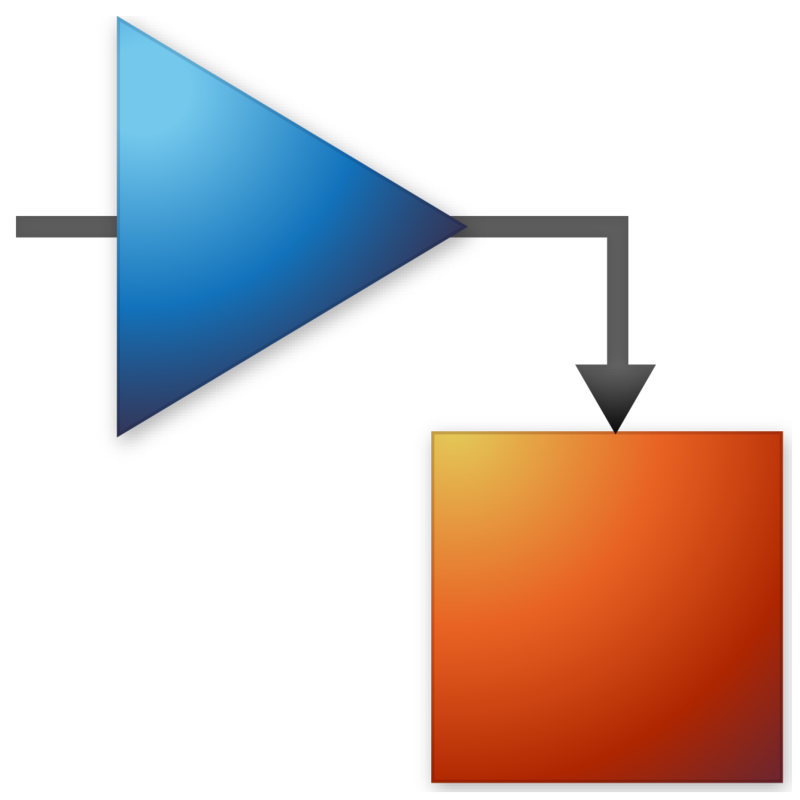
\includegraphics[scale = 0.05]{figs/Selection_036.png}
\end{flushright}
Toolboxes to be used in this course are
\begin{enumerate}
\item Programming
\item Simulink
\item Mupad (Symbolic math toolbox)
\item Matlab Editer
\begin{itemize}
\item Functions
\item Structures
\item Object-Oriented
\item Level 1 \& 2 S-Functions
\end{itemize}
\item GUI development
\item Report Generation
\end{enumerate}
\end{frame}



\begin{frame}[shrink]
\frametitle{Plotting step response manually \attachfile{code/qazi.m}}
Instead of using the step command to plot \textcolor{cyan}{step response},
the following manual method can be used for better understanding:
\lstset{language=Matlab,%
    %basicstyle=\color{red},
    breaklines=true,%
    morekeywords={matlab2tikz},
    keywordstyle=\color{blue},%
    morekeywords=[2]{1}, keywordstyle=[2]{\color{black}},
    identifierstyle=\color{black},%
    stringstyle=\color{mylilas},
    commentstyle=\color{mygreen},%
    showstringspaces=false,%without this there will be a symbol in the places where there is a space
    numbers=left,%
    numberstyle={\tiny \color{black}},% size of the numbers
    numbersep=9pt, % this defines how far the numbers are from the text
    emph=[1]{for,end,break},emphstyle=[1]\color{red}, %some words to emphasise
    %emph=[2]{word1,word2}, emphstyle=[2]{style},    
}
\tiny{
%\begin{tcolorbox}[title=  ,width=9.85 cm]

\begin{tikzpicture}
\node [mybox2] (box){%
    \begin{minipage}{0.93\textwidth}
       \lstinputlisting{code/qazi.m}
    \end{minipage}
};
\node[fancytitle2, right=10pt] at (box.north west) {Step Response};
\node[fancytitle2, rounded corners] at (box.east) {$\spadesuit$};
\end{tikzpicture}%
%\end{tcolorbox}
}
\label{step}
 \hyperlink{what}{\beamergotobutton{Back to the slide 58}}
\end{frame}


%%%%%%%%%%%%%%%%%%%%%%%%%%%

\section{Lecture}
\subsection{Assignments}

\begin{frame}
\pagecolor{black}
\color{white}
\frametitle{Lectures \& Assignments for Matlab}
Press the pin to get lectures \& assignments 
\begin{itemize}
\item[\ding{40}] \textcolor{red}{Lecture 1}\attachfile{MIT/lec_01.pdf}
\begin{itemize}
\item[\ding{88}] \textcolor{mygreen}{Assignment 01}\attachfile{assig/ass1.pdf}
\end{itemize}
\item[\ding{40}] \textcolor{red}{Lecture 2}\attachfile{MIT/lec_02.pdf}
\begin{itemize}
\item[\ding{88}] \textcolor{mygreen}{Assignment 02}\attachfile{assig/ass2.pdf}
\end{itemize}
\item[\ding{40}] \textcolor{red}{Lecture 3}\attachfile{MIT/lec_03.pdf}
\begin{itemize}
\item[\ding{88}] \textcolor{mygreen}{Assignment 03}\attachfile{assig/ass3.pdf}
\end{itemize}
\item[\ding{40}] \textcolor{red}{Lecture 4}\attachfile{MIT/lec_04.pdf}
\begin{itemize}
\item[\ding{88}] \textcolor{mygreen}{Assignment 04}\attachfile{assig/ass4.pdf}
\end{itemize}
\item[\ding{40}] \textcolor{red}{Lecture 5}\attachfile{MIT/lec_05.pdf}
\item[\ding{40}] \textcolor{blue}{mat Files that could be used} \attachfile{assig/my.zip}
\item[\ding{40}] \textcolor{orange}{m-Files that could be used} \attachfile{assig/HH.zip}
\end{itemize}
\end{frame}


%%%%%%%%%%%%%%%%%%%%%%%%%%%%%%%
\section{Labs}




\subsection{flowchart}

\begin{frame}
\frametitle{Flow Chart}
\tikzstyle{startstop} = [rectangle, rounded corners, minimum width=1.8cm, minimum height=0.5cm,text centered, draw=black, fill=red!30]
\tikzstyle{io} = [trapezium, trapezium left angle=70, trapezium right angle=110, minimum width=1.8cm, minimum height=0.5cm, text centered, draw=black, fill=blue!30]
\tikzstyle{process} = [rectangle, minimum width=1.8cm, minimum height=0.6cm, text centered, draw=black, fill=orange!30]
\tikzstyle{decision} = [diamond, minimum width=1.2cm, minimum height=0.3cm, text centered, draw=black, fill=green!30]
\tikzstyle{arrow} = [thick,->,>=stealth]
\begin{center}
\tiny{
\begin{tikzpicture}[node distance=1.3cm]
\node (start) [startstop] {Start};
\node (in1) [io, below of=start] {Input};
\node (pro1) [process, below of=in1] {Process 1};
\node (dec1) [decision, below of=pro1] {Decision 1};
\node (pro2a) [process, below of=dec1, yshift=-0.15cm] {Process 2a};
\node (pro2b) [process, right of=dec1, xshift=2cm] {Process 2b};
\node (out1) [io, below of=pro2a] {Output};
\node (stop) [startstop, below of=out1] {Stop};
\draw [arrow] (start) -- (in1);
\draw [arrow] (in1) -- (pro1);
\draw [arrow] (pro1) -- (dec1);
\draw [arrow] (dec1) -- (pro2a);
\draw [arrow] (dec1) -- (pro2b);;
\draw [arrow] (dec1) -- node[anchor=east] {yes} (pro2a);
\draw [arrow] (dec1) -- node[anchor=south] {no} (pro2b);
\draw [arrow] (pro2a) -- (out1);
\draw [arrow] (out1) -- (stop);
\draw [arrow] (pro2b) |- (pro1);
\end{tikzpicture}}
\end{center}
\end{frame}

\begin{frame}[shrink]
\frametitle{Flow Chart}
\pagestyle{empty}

\centering
% Define block styles
\tikzstyle{decision} = [diamond, draw, fill=blue!20, 
    text width=4.5em, text badly centered, node distance=3cm, inner sep=0pt]
\tikzstyle{block} = [rectangle, draw, fill=blue!20, 
    text width=5em, text centered, rounded corners, minimum height=4em]
\tikzstyle{line} = [draw, -latex']
\tikzstyle{cloud} = [draw, ellipse,fill=red!20, node distance=3cm,
    minimum height=2em]
    
\begin{tikzpicture}[node distance = 2cm, auto]
    % Place nodes
    \node [block] (init) {initialize model};
    \node [cloud, left of=init] (expert) {expert};
    \node [cloud, right of=init] (system) {system};
    \node [block, below of=init] (identify) {identify candidate models};
    \node [block, below of=identify] (evaluate) {evaluate candidate models};
    \node [block, left of=evaluate, node distance=3cm] (update) {update model};
    \node [decision, below of=evaluate] (decide) {is best candidate better?};
    \node [block, below of=decide, node distance=3cm] (stop) {stop};
    % Draw edges
    \path [line] (init) -- (identify);
    \path [line] (identify) -- (evaluate);
    \path [line] (evaluate) -- (decide);
    \path [line] (decide) -| node [near start] {yes} (update);
    \path [line] (update) |- (identify);
    \path [line] (decide) -- node {no}(stop);
    \path [line,dashed] (expert) -- (init);
    \path [line,dashed] (system) -- (init);
    \path [line,dashed] (system) |- (evaluate);
\end{tikzpicture}

\end{frame}


\begin{frame}
\frametitle{Computational Complexity Classes}
\tiny{
\begin{tikzpicture}
\pgftransformscale{.5}

%%% HELP LINES - uncomment to design/extend
% \draw[step=1cm,gray,very thin] (-10,0) grid (10,12);
% \node at (0,0) {\textbf{(0,0)}};

%% Horizontal bar
\draw[very thick] (10,0) -- (-10,0);

% LOG TIME
\draw (-1,0) parabola bend (0,2) (1,0) ;
\node at (0,1) {
	\begin{tabular}{c}
	LOG \\ Time
	\end{tabular}
};

% LOG SPACE
\draw (-2,0) parabola bend (0,3.5) (2,0);
\node at (0,2.5) {
	\begin{tabular}{c}
	LOG \\ Space
	\end{tabular}
};

% PTIME
\draw (-3,0) parabola bend (0,4.5) (3,0);
\node at (0,4) {PTIME};

% NP
\draw[dotted] (-4,0) parabola bend (2,6) (4.5,0);
\node[rotate=-45] at (3,3.5) {NPTIME};

% NP-complete
\node[circle,dotted,draw] at (2,5) {NPC};

% Co-NP
\draw[dashed] (4,0) parabola bend (-2,6) (-4.5,0);
\node[rotate=45] at (-2.5,4) {co-NPTIME};

% PSPACE
\draw (-6,0) parabola bend (0,7.2) (6,0);
\node at (0,6.5) {PSPACE};

% EXPTIME
\draw (-7,0) parabola bend (0,8.5) (7,0);
\node at (0,8) {EXPTIME};

% EXPTIME
\draw (-8,0) parabola bend (0,9.5) (8,0);
\node at (0,9) {EXPSPACE};

% ELEMENTARY
\draw (-9,0) parabola bend (0,11.5) (9,0);
\node at (0,10.5) {$\vdots$};
\node[anchor=north] at (0,11.4) {
	\begin{tabular}{c}
		ELEMENTARY \\
		$\vdots$ \\
		2EXPTIME
	\end{tabular}
};

% RECURSIVE
\draw[very thick] (-9.5,0) parabola bend (0,12.5) (9.5,0);
\node at (0,12) {MATLAB};
\end{tikzpicture}}
\end{frame}

\subsection{Lab Architecture}

\begin{frame}
\frametitle{Lab1 \\{\large Learn to Record and Share Your \\ Results Electronically}}
\begin{itemize}
\item Learn how to make a website and put your results on it
\begin{itemize}
\item Website files must not be path dependent, i.e, if I copy\
them to any location such as a USB, or different directory,
the website must still work
\item The main file of the website must be index.html
\end{itemize}
\item Many tools are available, but a good cross-platform open source
software is kompozer available from \url{http://www.kompozer.net/}
\end{itemize}
\end{frame}



\begin{frame}
\frametitle{Lab1 \\{\large Learn to Extend Existing Work in a \\ Controls Topic}}
Make groups, pick a research topic, create a website with following
headings:
\begin{enumerate}
\item Introduction
\item Technical Background
\item Expected Experiments
\item Expected Results
\item Expected Conclusions
\end{enumerate}
Present your website. Every group member will be quizzed randomly.
Your final work will count towards your lab exam.
\end{frame}


\begin{frame}
\frametitle{Matlab}
\begin{enumerate}
\item {\bf General}
  \begin{itemize}
  \item {\bf Info on Matlab} \textcolor{blue}{ver, version, license, computer, path}
  \item {\bf Initialization}  \textcolor{blue}{clc, clear, close all}
  \item {\bf Info on workspace} \textcolor{blue}{whos, ans}
  \item {\bf Help} \textcolor{blue}{help, doc}
  \item {\bf Feedback} \textcolor{blue}{disp, ;}
  \end{itemize}
\item {\bf Mathematical operators/functions/data types}
  \begin{itemize}
  \item {\bf Standard operators} \textcolor{black}{+  -  *  /  $\hat{}$}
  \item {\bf Point-wise operators}  \textcolor{black}{*.   /.   $\hat{.}$}
  \item {\bf Bit-wise operators} \textcolor{blue}{bitand,bitor}
  \item {\bf Logical operators} \textcolor{blue}{\&\&, ||}
  \item {\bf Transcedental functions} \textcolor{blue}{exp, sin, cos, tan, acos, asin, atan, log, log10}
  \item {\bf Complex} \textcolor{blue}{j, abs, angle}
  \item {\bf Data types}
    \begin{itemize}
    \item {\bf numeric} \textcolor{blue}{int8(16,32,64), uint8(16,32,64), single, double}
    \item {\bf string} \textcolor{blue}{char}
    \item {\bf arrays, matrices} \textcolor{blue}{size} [] () : ; ' (1-based)
    \end{itemize}
  \end{itemize}
\end{enumerate}
\end{frame}

\begin{frame}
\frametitle{Matlab}
\begin{enumerate}
\item {\bf Flow Control}
  \begin{itemize}
  \item {\bf Loops} \textcolor{blue}{for, while, end}
  \item {\bf Conditional}  \textcolor{blue}{if, end}
  \item {\bf Relational} < > <= >= == ~=
  \end{itemize}
\item {\bf Visualization (2D and 3D plots)}
  \begin{itemize}
  \item {\bf 2D} \textcolor{blue}{plot, stem}
  \item {\bf 3D}  \textcolor{blue}{plot3, mesh, surf}
  \item {\bf general} \textcolor{blue}{xlabel, ylabel, title, subplot, grid, hold, colormap, colorbar}
  \end{itemize}
\end{enumerate}
\end{frame}

\begin{frame}
\frametitle{Matlab \\ {\small Extra}}
\begin{enumerate}
\item {\bf Symbolic math} \textcolor{blue}{syms, solve}
\item {\bf File I/O}
  \begin{itemize}
  \item {\bf Open/close} \textcolor{blue}{fopen, fclose}
  \item {\bf Text}  \textcolor{blue}{fprintf, fscanf (also: textread, textscan, dlmread,
dlmwrite, csvread)}
  \item {\bf Binary} \textcolor{blue}{fread, fwrite}
  \item {\bf Excel} \textcolor{blue}{xlsread, xlswrite}
  \item {\bf Sound} \textcolor{blue}{wavread, wavwrite}
  \item {\bf image} \textcolor{blue}{imread, imwrite}
  \item {\bf Video} \textcolor{blue}{VideoReader}
  \end{itemize}
\item {\bf Graphical User Interface (GUI)} \textcolor{blue}{guide}
\item {\bf Signal processing}
  \begin{itemize}
  \item {\bf Commands} \textcolor{blue}{fft, freqs, freqz, filter}
  \item {\bf Tools}  \textcolor{blue}{sptool, fdatool}
  \item {\bf Play sound} \textcolor{blue}{sound, soundsc}
  \item {\bf View image} \textcolor{blue}{imview, imagesc}
  \end{itemize}
\end{enumerate}
\end{frame}

\subsection{Introduction}

\begin{frame}
\frametitle{Matlab Interfaces \\ {\small Introduction}}
\begin{tikzpicture}[%
  % common options for blocks:
  block/.style = {draw, fill=blue!30, align=center, anchor=west,
              minimum height=0.65cm, inner sep=0},
  % common options for the circles:
  ball/.style = {circle, draw, align=center, anchor=north, inner sep=0}]
\node[anchor=south west,inner sep=0] at (0,0) {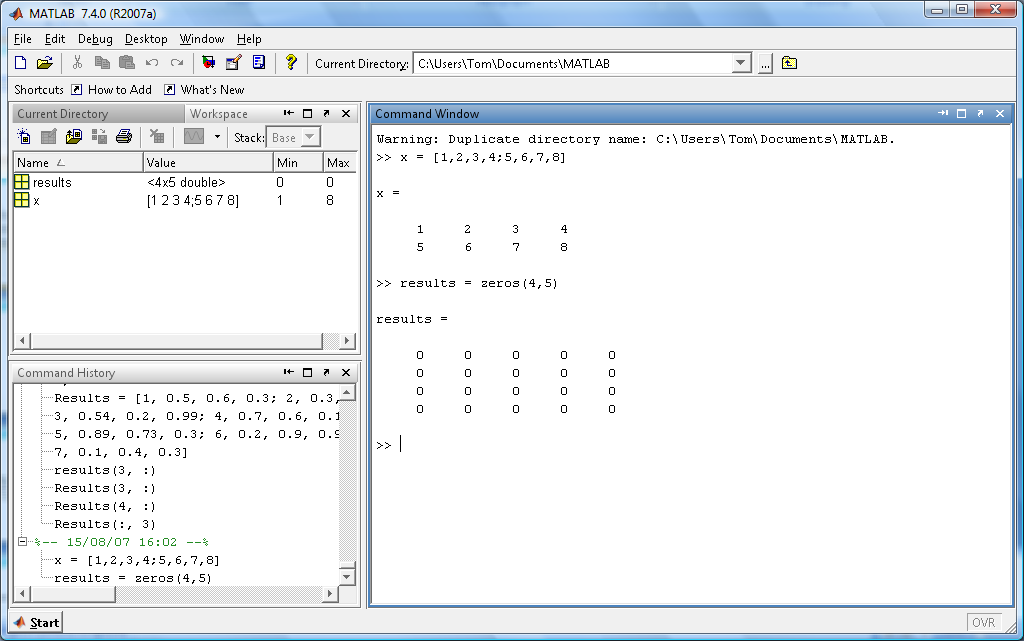
\includegraphics[width=\textwidth]{figs/asd.png}};
\node[draw, fill=purple!20] at (1.5,3.5) {Workspace};
\node[draw,align=center, fill=red!20] at (6.6,1.5) {Command Window \\ Console};
\node[draw,text width=1.5cm,fill=green!10] at (1.5, 1.2) {History};
\end{tikzpicture}
\end{frame}



\begin{frame}
\frametitle{Matlab \\ {\small Window Components}}
\begin{itemize}
\item[\ding{36}] Command Prompt - MATLAB commands are entered here.
\item[\ding{36}] Workspace - Displays any variables created (Matrices, Vectors, Singles, etc.)
\item[\ding{36}] Command History - Lists all commands previously entered.
\end{itemize}
\begin{itemize}
\item Double clicking on a variable in the Workspace will open an Array Editor. This will give you an Excel-like view of your data.
\end{itemize}
\end{frame}

\begin{frame}
\frametitle{Matlab \\ {\small Interface}}
\begin{itemize}
\item[\ding{39}] Pressing the up arrow in the command window will bring up the last command entered.
  \begin{itemize}
  \item[*] This saves you time when things go wrong
  \end{itemize}
\item[\ding{39}] If you want to bring up a command from some time in the past type the first letter and press the up arrow.
\item[\ding{39}] The current working directory should be set to a directory of your own 
\end{itemize}
\end{frame}

\begin{frame}
\frametitle{Matlab \\ {\small Creating Variables}}
\begin{itemize}
\item Variables
  \begin{itemize}
  \item[*] Names
    \begin{itemize}
     \item Can be any string of upper and lower case letters along with numbers and underscores but it must begin with a letter 
     \item Reserved names are IF, WHILE, ELSE, END, SUM, etc.
     \item Names are case sensitive
    \end{itemize}
  \item[*] Value
    \begin{itemize}
     \item This is the data the is associated to the variable; the data is accessed by using the name.
    \end{itemize}
  \item[*] This is the data the is associated to the variable; the data is accessed by using the name.
     \begin{itemize}
     \item Re-assignment is done silently-there are no warnings if you overwrite a variable with something of a different type.
    \end{itemize}
  \end{itemize}
\end{itemize}
\end{frame}

\begin{frame}
\frametitle{Matlab \\ {\small Some Useful Commands}}
\begin{columns}
\column{0.2\textwidth}
\textcolor{blue}{what \\
dir \\
ls \\
type test \\
delete test \\
cd a: \\
chdir a: \\
pwd \\
which test}
\column{0.7\textwidth}
List all m-files in current directory \\
List all files in current directory \\
Same as dir \\
Display test.m in command window \\
Delete test.m \\
Change directory to a: \\
Same as cd \\
Show current directory \\
Display current directory path to test.m
\end{columns}
\end{frame}

\subsubsection{Math}


\begin{frame}
\frametitle{Matlab \\ {\small Math}}
* \quad MATLAB can do simple math just as a calculator.
\begin{table}
\begin{tabular}{| l | c | c | }
\hline
Operation & Symbol & Example  \\
\hline \hline
Addition, a + b & + & 3 + 22  \\ 
\hline
Subtraction, a $-$ b & - & 90 - 44 \\
\hline
Multiplication, a$\times$b & * & pi*3.84 \\
\hline
Division, a $\div$ b & / or $\backslash$ & 56/8=8$\backslash$56  \\
\hline
Exponentiation, $a^b$ & $\hat{}$ & 2$\hat{}$16 \\
\hline
\end{tabular}
\end{table}
\end{frame}

\begin{frame}
\frametitle{Matlab \\ {\small Special Variables }}
\begin{description}
\item[\textcolor{blue}{ans}] Default variable name for results
\item[\textcolor{blue}{pi}] Value of $\pi$
\item[\textcolor{blue}{inf}] $\infty$
\item[\textcolor{blue}{NaN}] Not a number e.g. 0/0
\item[\textcolor{blue}{i} \& \textcolor{blue}{j}] i=j=$\sqrt{-1}$
\item[\textcolor{blue}{eps}] Smallest incremental number
\item[\textcolor{blue}{realmin}] The smallest usable positive real number
\item[\textcolor{blue}{realmax}] The largest usable positive real number
\end{description}
\end{frame}


\subsubsection{Variable Declaration}
\begin{frame}
\frametitle{Matlab \\ {\small Creating Variables}}
\begin{itemize}
\item Single Values
  \begin{itemize}
  \item To assign a value to a variable use the equal symbol '=' \\ >> \textcolor{mygreen}{A=32}
  \item To make another variable equal to one already entered \\ >> \textcolor{mygreen}{B=A}
  \item The new variable is not updated as you change the original value
  \item The value of two variables can be added together, and the result displayed... \\ >> \textcolor{mygreen}{A=10} \\>> \textcolor{mygreen}{A+A}
  \item ...or the result can be stored in another variable \\>> \textcolor{mygreen}{A=10} \\ >> \textcolor{mygreen}{B=A+A}
  \end{itemize}
\end{itemize}
\noindent\makebox[\linewidth]{\rule{10 cm}{0.1pt}}
Note: using ; suppresses output
\end{frame}

\begin{frame}
\frametitle{Matlab \\ {\small Vectors}}
\begin{itemize}
\item A vector is a list of numbers
  \begin{itemize}
  \item Use square brackets \textcolor{red}{\large [ ]} to contain the numbers \\ 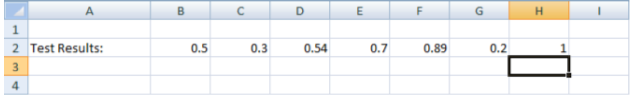
\includegraphics[scale = 0.35]{figs/Selection_015.png}
  \end{itemize}
\item To create a row vector use ‘\textcolor{red}{\huge ,}’ to separate the content
\item To create a column vector use ‘\textcolor{red}{\huge ;}’ to separate the content \\ \begin{center} 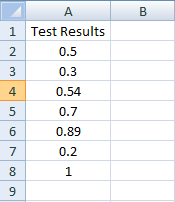
\includegraphics[scale = 0.35]{figs/Selection_017.png} \end{center}
\item A row vector can be converted into a column vector by using the transpose operator \textcolor{red}{\huge '}
\end{itemize}
\end{frame}

\begin{frame}
\frametitle{Matlab \\ {\small Matrices}}
\begin{itemize}
\item A MATLAB matrix is a rectangular array of numbers
  \begin{itemize}
  \item Scalars and vectors are regarded as special cases of matrices
  \item MATLAB allows you to work with a whole array at a time
  \end{itemize}
\item You can create matrices (arrays) of any size using a combination of the methods for creating vectors
\item List the numbers using '\textcolor{red}{\huge ,}' to separate each column and then '\textcolor{red}{\huge ;}' to define a new row
\end{itemize}
\begin{figure}[!tbp]
\centering
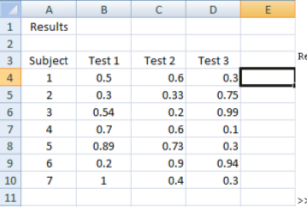
\includegraphics[scale = 0.32]{figs/Selection_018.png}
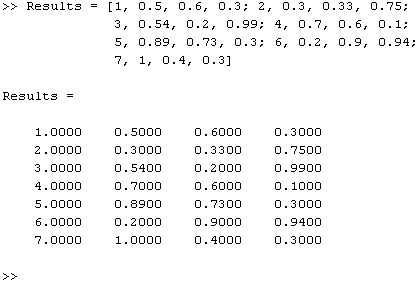
\includegraphics[scale = 0.3]{figs/Selection_018a.png}
\end{figure}
\end{frame}

\begin{frame}
\frametitle{Matlab \\ {\small Matrices}}
\begin{itemize}
\item You can also use built in functions to create a matrix
  \begin{itemize}
  \item >> \textcolor{mygreen}{A = zeros(2, 4)} \\
		creates a matrix called A with 2 rows and 4 columns 	containing the value 0
  \item >> \textcolor{mygreen}{A = zeros(5)} or >> \textcolor{mygreen}{A = zeros(5, 5)}  \\
		creates a matrix called A with 5 rows and 5 columns
  \end{itemize}
\item You can also use:
  \begin{itemize}
  \item >> \textcolor{mygreen}{ones(rows, columns)}
  \item >> \textcolor{mygreen}{rand(rows, columns)}
  \end{itemize}
\end{itemize}
\noindent\makebox[\linewidth]{\rule{10 cm}{0.1pt}}
Note: MATLAB always refers to the first value as the number of Rows then the second as the number of Columns
\noindent\makebox[\linewidth]{\rule{10 cm}{0.1pt}}
\end{frame}


\begin{frame}
\frametitle{Matlab \\ {\large Accessing Matrix Elements}}
\begin{figure}[!tbp]
\centering
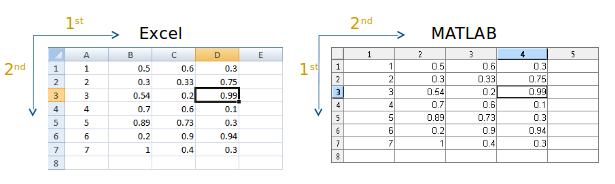
\includegraphics[scale = 0.46]{figs/Selection_012a.png}
\end{figure}
\begin{itemize}
\item To access Subject 3's result for Test 3
  \begin{itemize}
  \item In Excel (Column, Row): \\ \begin{center} D3 \end{center}
  \item In Matlab (Row,Column): \\ \begin{center} >>\textcolor{mygreen}{results(3, 4)} \end{center}
  \end{itemize}
\item The referenced element can also be changed \\ \begin{center} >>\textcolor{mygreen}{results(3, 4) = 10} or \\
>> \textcolor{mygreen}{results(3,4) = results(3,4) * 100} \end{center}
\end{itemize}
\end{frame}

\subsubsection{Matrices \& Arrays} 

\begin{frame}[fragile]
\frametitle{Matlab \\ {\small Array and Matrices}}
Vectors array are defined as
\begin{tcolorbox}[title= ,width=9.85 cm]
\begin{lstlisting}[language=C++]
>> v = [1, 2, 4, 5] 
>> w = [1; 2; 4; 5]
\end{lstlisting}
\end{tcolorbox}
Matrices (2D arrays) defined similarly
\begin{tcolorbox}[title= ,width=9.85 cm]
\begin{lstlisting}[language=C++,basicstyle=\ttfamily,keywordstyle=\color{red}]
>> A = [1,2,3;4,-5,6;5,-6,7]
\end{lstlisting}
\end{tcolorbox}
\end{frame}




\begin{frame}
\frametitle{Matlab \\ {\small Array and Matrices}}
\begin{itemize}
\item[\textcolor{blue}{zeros}] creates an array of all zeros, Ex: x = zeros(3,2)
\item[\textcolor{blue}{ones}] creates an array of all ones, Ex: x = ones(2)
\item[\textcolor{blue}{eye}] creates an identity matrix, Ex: x = eye(3)
\item[\textcolor{blue}{rand}] generates uniformly distributed random numbers in [0,1]
\item[\textcolor{blue}{diag}] diagonal matrices and diagonal of a matrix
\item[\textcolor{blue}{size}] returns array dimensions
\item[\textcolor{blue}{length}] returns length of a vector (row or column)
\item[\textcolor{blue}{det}] Matrix determinant
\item[\textcolor{blue}{inv}] Matrix inverse
\item[\textcolor{blue}{eig }] evaluates eigenvalues and eigenvectors
\item[\textcolor{blue}{rank}] rank of a matrix
\item[\textcolor{blue}{find}] searches for the given values in an array/matrix
\end{itemize}
\end{frame}

\begin{frame}[fragile]
\frametitle{Matlab \\ {\small Polynomial Example}}
Find polynomial roots:
$$1.2x^3+0.5x^2+4x+10$$
\begin{tcolorbox}[title= ,width=9.85 cm]
x=[1.2,0.5,4,10]
\begin{lstlisting}[language=C++]
>> x=[1.2,0.5,4,10]
>> x
      1.2 0.5 4 10
>>roots(x)
\end{lstlisting}
\end{tcolorbox}
\end{frame}





\subsection{Flow Control}

\begin{frame}
\frametitle{Matlab \\ {\small Flow Control}}
\begin{itemize}
\item[\textcolor{gray}{\ding{56}}] MATLAB has five flow control statements
\begin{itemize}
\item[-] \textcolor{red}{if} statements
\item[-] \textcolor{red}{switch} statements
\item[-] \textcolor{red}{for} loops
\item[-] \textcolor{red}{while} loops
\item[-] \textcolor{red}{break} statements
\end{itemize}
\end{itemize}
\end{frame}

\subsubsection{a) if statement}

\begin{frame}[fragile]
\frametitle{Matlab \\ {\small if Statements}}
\begin{columns}
    \begin{column}{0.49\textwidth}
        \begin{itemize}
         \item[\ding{59}] The general form of the '\textcolor{red}{if}' statement is 
         \end{itemize}
\begin{tcolorbox}
\scriptsize{
\begin{lstlisting}[language=C++,basicstyle=\ttfamily,keywordstyle=\color{red}]
>> if expression
>> ...
>> elseif expression
>> ...
>> else
>> ...
>> end
\end{lstlisting} }
\end{tcolorbox}
      \end{column}
    \begin{column}{0.5\textwidth}
        \begin{itemize}
         \item[\ding{59}] Example 1: 
         \end{itemize}
\small{
\begin{lstlisting}[language=C++,basicstyle=\ttfamily,keywordstyle=\color{red}]
>> if i == j
>>      a(i,j) = 2;
>> elseif i >= j
>>      a(i,j) = 1;
>> else
>>      a(i,j) = 0;
>> end
\end{lstlisting} }
 \begin{itemize}
         \item[\ding{59}] Example 2: 
         \end{itemize}
\scriptsize{
\begin{lstlisting}[language=C++,basicstyle=\ttfamily,keywordstyle=\color{red}]
>> if (attn>0.9)&(grade>60)
>>    pass = 1;
>> end
\end{lstlisting} }
    \end{column}
\end{columns}
\end{frame}

\subsubsection{b) switch statement}

\begin{frame}[fragile]
\frametitle{Matlab \\ {\small switch Statements}}
 \begin{itemize}
         \item[\ding{60}] \textcolor{red}{switch} Switch among several cases based on expression
         \end{itemize}
\begin{columns}
    \begin{column}{0.49\textwidth}
        \begin{itemize}
         \item[\ding{60}] The general form of the '\textcolor{red}{if}' statement is 
         \end{itemize}
\begin{tcolorbox}
\scriptsize{
\begin{lstlisting}[language=C++,basicstyle=\ttfamily,keywordstyle=\color{red}]
>> switch switch_expr
>>   case case_expr1
>>           ...
>>   case case_expr2
>>           ...
>>   otherwise
>>           ... 
>> end
\end{lstlisting} }
\end{tcolorbox}
      \end{column}
    \begin{column}{0.5\textwidth}
        \begin{itemize}
         \item[\ding{60}] Example 
         \end{itemize}
\tiny{
\begin{lstlisting}[language=C++,basicstyle=\ttfamily,keywordstyle=\color{red}]
>> x = 2, y = 3;
>> switch x
>>  case x==y
>>   disp('x and y are equal');
>>  case x>y
>>   disp('x is greater than y');
>>  otherwise
>>    disp('x is less than y');
>> end
x is less than y
\end{lstlisting}}
\textcolor{red}{Note: Unlike C, MATLAB doesn't need
BREAKs in each case}
    \end{column}
\end{columns}
\end{frame}

\subsubsection{c) foor loop}

\begin{frame}[fragile]
\frametitle{Matlab \\ {\small For loops}}
 \begin{itemize}
         \item[\ding{60}] \textcolor{red}{for} Repeat statements a specific number of times
         \end{itemize}
\begin{columns}
    \begin{column}{0.58\textwidth}
        \begin{itemize}
         \item[\ding{60}] The general form of the '\textcolor{red}{for}' statement is 
         \end{itemize}
\begin{tcolorbox}
\scriptsize{
\begin{lstlisting}[language=C++,basicstyle=\ttfamily,keywordstyle=\color{red}]
>> for variable=expression
>>   ...
>>   ...
>> end
\end{lstlisting} }
\end{tcolorbox}
      \end{column}
    \begin{column}{0.38\textwidth}
        \begin{itemize}
         \item[\ding{60}] Example 1:
         \end{itemize}
\tiny{
\begin{lstlisting}[language=C++,basicstyle=\ttfamily,keywordstyle=\color{red}]
>> for x = 0:0.05:1
>>  printf('\%d\n',x);
>> end
\end{lstlisting}}
\large{
 \begin{itemize}
         \item[\ding{60}] Example 2:
         \end{itemize}}
\tiny{
\begin{lstlisting}[language=C++,basicstyle=\ttfamily,keywordstyle=\color{red}]
>> a = zeros(n,m);
>> for i = 1:n
>>   for j = 1:m
>>       a(i,j) = 1/(i+j);
>>   end
>> end
\end{lstlisting}}
    \end{column}
\end{columns}
\end{frame}

\subsubsection{d) while loop}

\begin{frame}[fragile]
\frametitle{Matlab \\ {\small While loops}}
 \begin{itemize}
         \item[\ding{61}] \textcolor{red}{while} Repeat statements an indefinite number of times
         \end{itemize}
\begin{columns}
    \begin{column}{0.58\textwidth}
        \begin{itemize}
         \item[\ding{61}] The general form of the '\textcolor{red}{while}' statement is 
         \end{itemize}
\begin{tcolorbox}
\scriptsize{
\begin{lstlisting}[language=C++,basicstyle=\ttfamily,keywordstyle=\color{red}]
>> while expression
>>    ...
>>    ...
>> end
\end{lstlisting} }
\end{tcolorbox}
      \end{column}
    \begin{column}{0.38\textwidth}
        \begin{itemize}
         \item[\ding{61}] Example 1:
         \end{itemize}
\tiny{
\begin{lstlisting}[language=C++,basicstyle=\ttfamily,keywordstyle=\color{red}]
>> n = 1;
>> y = zeros(1,10);
>> while n <= 10
>>     y(n) = 2*n/(n+1);
>>     n = n+1;
>> end
\end{lstlisting}}
\large{
 \begin{itemize}
         \item[\ding{61}] Example 2:
         \end{itemize}}
\tiny{
\begin{lstlisting}[language=C++,basicstyle=\ttfamily,keywordstyle=\color{red}]
>> x = 1;
>> while x
>>   %execute statements
>> end
\end{lstlisting}}
    \end{column}
\end{columns}
\textcolor{red}{Note: In MATLAB '1' is
synonymous to TRUE and '0' is
synonymous to FALSE}
\end{frame}


\begin{frame}[fragile]
\frametitle{Matlab \\ {\small break function}}
\begin{itemize}
\item[\ding{63}] \textcolor{red}{break} terminates the execution of \textcolor{red}{for} and \textcolor{red}{while} loops
\item[\ding{63}] In nested loops, \textcolor{red}{break} terminates from the innermost loop only
\end{itemize}

\begin{itemize}
\item[\ding{64}] Example
\end{itemize}
\begin{lstlisting}[language=C++,basicstyle=\ttfamily,keywordstyle=\color{red}]
>> y = 3;
>> for x = 1:10
>>    printf('%5d',x);
>>    if (x>y)
>>       break;
>>    end
>> end
      1  2  3  4
\end{lstlisting}
\end{frame}



\begin{frame}
\frametitle{Matlab}
\framesubtitle{Efficient Programming $_{\tiny \insertframenumber/\inserttotalframenumber}$}
\begin{itemize}
\item Avoid using nested loops as far as possible
\item In most cases, one can replace nested loops with efficient matrix
manipulation.
\item Preallocate your arrays when possible
\item MATLAB comes with a huge library of in-built functions, use them
when necessary
\item Avoid using your own functions, MATLAB’s functions are more likely
to be efficient than yours.
\end{itemize}
\end{frame}





\section{Simulink}

\begin{frame}
\frametitle{Simulink}
\framesubtitle{Diagram Analogy to Simulink BLocks}
\pagestyle{empty}

\tikzstyle{int}=[draw, fill=blue!20, minimum size=2em]
\tikzstyle{init} = [pin edge={to-,thin,black}]
\centering
\begin{tikzpicture}[node distance=2.5cm,auto,>=latex']
    \node [int, pin={[init]above:$v_0$}] (a) {$\frac{1}{s}$};
    \node (b) [left of=a,node distance=2cm, coordinate] {a};
    \node [int, pin={[init]above:$d_0$}] (c) [right of=a] {$\frac{1}{s}$};
    \node [coordinate] (end) [right of=c, node distance=2cm]{};
    \path[->] (b) edge node {$a$} (a);
    \path[->] (a) edge node {$v$} (c);
    \draw[->] (c) edge node {$d$} (end) ;
\end{tikzpicture}


\tikzstyle{block} = [draw,fill=blue!20,minimum size=2em]
% diameter of semicircle used to indicate that two lines are not connected
\def\radius{.7mm} 
\tikzstyle{branch}=[fill,shape=circle,minimum size=3pt,inner sep=0pt]

\begin{tikzpicture}[>=latex']

    % Draw blocks, inputs and outputs
    \foreach \y in {1,2,3,4,5} {
        \node at (0,-\y) (input\y) {$i_\y$};
        \node[block] at (2,-\y) (block\y) {$f_\y$};
        \draw[->] (input\y) -- (block\y);
        \draw[->] (block\y.east) -- +(0.5,0);
    }
    \node[block] at (2,-6) (block6) {$f_6$};
    \draw[->] (block6.east) -- +(0.5,0);

    % Calculate branch point coordinate
    \path (input1) -- coordinate (branch) (block1);

    % Define a style for shifting a coordinate upwards
    % Note the curly brackets around the coordinate.
    \tikzstyle{s}=[shift={(0mm,\radius)}]
    % It would be natural to use the yshift or xshift option, but that does
    % not seem to work when shifting coordinates.

    \draw[->] (branch) node[branch] {}{ % draw branch junction
            \foreach \c in {2,3,4,5} {
                % Draw semicircle junction to indicate that the lines are
                % not connected. The intersection between the lines are
                % calculated using the convenient -| syntax. Since we want
                % the semicircle to have its center where the lines intersect,
                % we have to shift the intersection coordinate using the 's'
                % style to account for this.
                [shift only] -- ([s]input\c -| branch) arc(90:-90:\radius)
                % Note the use of the [shift only] option. It is not necessary,
                % but I have used it to ensure that the semicircles have the
                % same size regardless of scaling.
            }
        } |- (block6);
\end{tikzpicture}

\end{frame}


\begin{frame}
\frametitle{Lab2 \\{\large Mathematical Modeling of Motor}}
\begin{itemize}
\item The model we will use will be for a DC motor as given
in this slides on \hyperlink{motor}{\beamergotobutton{Back to Motor Modelling Slide}}
\item Use the following default values for the 6 constants needed to
model the DC motor:
\end{itemize}
\begin{center}
  \begin{tabular}{ | l | c | r |}

    \hline
   $K_m$ & 0.01 & Nm/Amp \\ \hline
    $K_b$ & 0.01 & V/rad/s \\ \hline 
    L & 0.5 & H \\ \hline
    R & 1 & $\omega$ \\ \hline
J & 0.01 &kg \ $m^2$ \\ \hline
b &0.1 &N \ m \ s \\
    \hline
  \end{tabular}
\end{center}
\begin{itemize}
\item Enter in Matlab
\end{itemize}

\label{motor1}
\end{frame}

\begin{frame}
\frametitle{Lab2 \\{\large Mathematical Modeling}}
\begin{figure}[!tbp]
  \begin{minipage}[t]{0.2\textwidth}
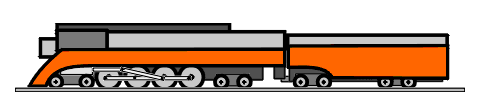
\includegraphics[scale = 0.28]{figs/Selection_037.png}
    \caption{Train system}
  \end{minipage}
  \hfill
  \begin{minipage}[t]{0.52\textwidth}
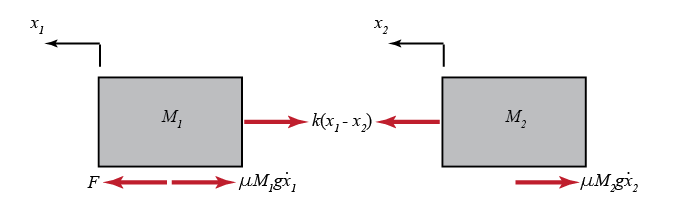
\includegraphics[scale = 0.25]{figs/Selection_038.png}
    \caption{Free body diagram}
  \end{minipage}
\end{figure}
In this example, we will consider a toy train consisting of an engine and a car. Assuming that the train only travels in one dimension (along the track), we want to apply control to the train so that it starts and comes to rest smoothly, and so that it can track a constant speed command with minimal error in steady state.
\end{frame}

\begin{frame}
\frametitle{Lab2 \\{\large Mathematical Modeling}}
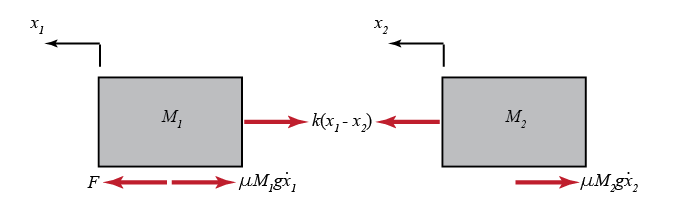
\includegraphics[scale = 0.45]{figs/Selection_038.png}

\begin{align*}
 \Sigma F_1 = F - k(x_1 - x_2) - \mu M_1 g \dot{x}_1 = M_1 \ddot{x}_1 \  \text{(1)}\\
 \Sigma F_2 = k(x_1 - x_2) - \mu M_2 g \dot{x}_2 = M_2 \ddot{x}_2  \ \text{(2)}
\end{align*}
\end{frame}

\begin{frame}
\frametitle{Lab2 \\{\large Mathematical Modeling in Simulink}}
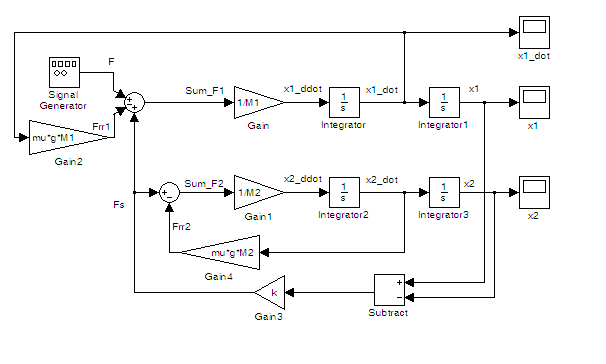
\includegraphics[scale = 0.52]{figs/Selection_039.png}
\\
Parameters are:
$M_1$=1 kg; $M_2$=0.5kg; k=1; F=1; $\mu$=0.02; g=9.8; 
\end{frame}


%%%%%%%%%%%%%%%%%%%%%%%%%%%%%%%%%%%%%%%%%%%%%%%%%%%%%




%%%%%%%%%%%%%%%%%%%%%%%%%%%%%%%%%%%%%%%%%


\section{Practice}
\subsection{Example 1} 

\begin{frame}[fragile]
\frametitle{Example 1}
\begin{itemize}
\item[\ding{89}] Let x[n] be the input to a non causal FIR filter, with filter
coefficients h[n]. Assume both the input values and the filter
coefficients are stored in column vectors x,h and are given to
you. Compute the output values y[n] for n = 1,2,3 where
\end{itemize}
\begin{align*}
\centering
y[n]=\sum_{k=0}^{19}h[k]x[n+k]
\end{align*}
\end{frame}

\subsubsection{Solution}

\begin{frame}[fragile]
\frametitle{Example 1}
\begin{columns}
    \begin{column}{0.58\textwidth}
        \begin{itemize}
         \item[\ding{71}] Method 1 
         \end{itemize}
\begin{tcolorbox}
\scriptsize{
\begin{lstlisting}[language=C++,basicstyle=\ttfamily,keywordstyle=\color{red}]
>>y = zeros(1,3);
>>for n = 1:3
>>   for k = 0:19
>>         y(n)= y(n)+h(k)*x(n+k);
>>   end
>>end
\end{lstlisting} }
\end{tcolorbox}
      \end{column}
    \begin{column}{0.38\textwidth}
        \begin{itemize}
         \item[\ding{71}] Method 2 (avoids inner loop):
         \end{itemize}
\tiny{
\begin{lstlisting}[language=C++,basicstyle=\ttfamily,keywordstyle=\color{red}]
>>y = zeros(1,3);
>>for n = 1:3
>>   y(n) = h'*x(n:(n+19));
>>end
\end{lstlisting}}
    \end{column}
\end{columns}
\begin{itemize}
         \item[\ding{71}] Method 3 (avoids both the loops):
         \end{itemize}
\begin{lstlisting}[language=C++,basicstyle=\ttfamily,keywordstyle=\color{red}]
>> X= [x(1:20),x(2:21),x(3:22)];
>> y = h'*X
\end{lstlisting}
\end{frame}

\subsection{Example 2} 
\begin{frame}[fragile]
\frametitle{Example 2}
\begin{itemize}
\item[\ding{90}] Compute the value of the following function
\end{itemize}
\small{
\begin{align*}
y(n)=1^3*(1^3+2^3 )*(1^3+2^3+3^3 )*...*(1^3+2^3+ ...+n^3 )
\end{align*}}
for n = 1 to 20
\end{frame}

\subsubsection{Solution}

\begin{frame}[fragile]
\frametitle{Example 1}
\begin{columns}
    \begin{column}{0.58\textwidth}
        \begin{itemize}
         \item[\ding{73}] Method 1 
         \end{itemize}
\begin{tcolorbox}
\scriptsize{
\begin{lstlisting}[language=C++,basicstyle=\ttfamily,keywordstyle=\color{red}]
>>y = zeros(20,1);
>>y(1) = 1;
>>for n = 2:20
>>  for m = 1:n
>>    temp = temp+m^3;
>>  end
>>  y(n) = y(n-1)*temp;
>>  temp = 0
>>end
\end{lstlisting} }
\end{tcolorbox}
      \end{column}
    \begin{column}{0.48\textwidth}
        \begin{itemize}
         \item[\ding{73}] Method 2 (avoids inner loop):
         \end{itemize}
\tiny{
\begin{lstlisting}[language=C++,basicstyle=\ttfamily,keywordstyle=\color{red}]
>>y = zeros(20,1);
>>y(1) = 1;
>>for n = 2:20
>>  temp = 1:n;
>>  y(n) = y(n-1)*sum(temp.^3);
>>end
\end{lstlisting}}
    \end{column}
\end{columns}
\begin{itemize}
         \item[\ding{71}] Method 3 (avoids both the loops):
         \end{itemize}
\begin{lstlisting}[language=C++,basicstyle=\ttfamily,keywordstyle=\color{red}]
>>X = tril(ones(20)*diag(1:20));
>>x = sum(X.^3,2);
>>Y = tril(ones(20)*diag(x))+ ...
triu(ones(20)) - eye(20);
>>y = prod(Y,2);
\end{lstlisting}
\end{frame}

\subsection{Example 3}
\begin{frame}
\frametitle{Example 3}
{\bf Discriminant}:
$$x_{1,2}=\frac{-b\pm\sqrt{b^2-4ac}}{2a}$$
Write a program such that values are requested by user as input and solution is determined accordingly 
\end{frame}

\subsubsection{Solution}
\begin{frame}
\frametitle{Example 3}
\scriptsize{
\begin{tcolorbox}[title= Code ,width=9.85 cm]
\lstinputlisting{code/qazii.m}
\end{tcolorbox}}
\end{frame}

\subsection{other}
\begin{frame}[fragile]
\frametitle{Matlab Graphics}
\framesubtitle{Visualization of vector data is available $_{\tiny \insertframenumber/\inserttotalframenumber}$}
\begin{lstlisting}[language=C++]
>>x= -pi:0.1:pi; 
>>y=sin(x);
>>plot(x,y)
>>xlabel('x');
>>ylabel('y=sin(x)');
\end{lstlisting}
\begin{tcolorbox}[title= Code ,width=9.85 cm]
\lstinputlisting{code/qazih.m}
\end{tcolorbox}
\end{frame}





\begin{frame}[shrink]
\frametitle{Lab2 \\{\large Loops, conditional statements, functions}}
\small{
\begin{tcolorbox}[title=Conditional statements ,width=9.85 cm]
\lstinputlisting{code/qazib.m}
\end{tcolorbox}

\begin{tcolorbox}[title=loops ,width=9.85 cm]
\lstinputlisting{code/qazic.m}
\end{tcolorbox}
}
\end{frame}

\begin{frame}
\frametitle{Lab2 \\{\large Loops, conditional statements, functions}}
\tiny{
\begin{tcolorbox}[title=saving/loading workspace variables ,width=9.85 cm]
\lstinputlisting{code/qazid.m}
\end{tcolorbox}

\begin{tcolorbox}[title=functions ,width=9.85 cm]
\lstinputlisting{code/qazie.m}
\end{tcolorbox}
}
\end{frame}

\section{codes}
\subsection{Basics}

\begin{frame}
\frametitle{Printing Output}
\begin{tcolorbox}[title=,width=9.85 cm]
\lstinputlisting{code/hello_world.m}
\end{tcolorbox}
\end{frame}

\begin{frame}
\frametitle{Circle}
\begin{tcolorbox}[title=Drawing Circle in Matlab ,width=9.85 cm]
\lstinputlisting{code/circle.m}
\end{tcolorbox}
\end{frame}

\begin{frame}
\frametitle{Advance Programming}
\begin{tcolorbox}[title=,width=9.85 cm]
\lstinputlisting{code/myplot.m}
\end{tcolorbox}
\end{frame}

\subsection{Animation}

\begin{frame}
\frametitle{Animations in Matlab}
\begin{tcolorbox}[title= ,width=9.85 cm]
\lstinputlisting{code/mp.m}
\end{tcolorbox}
\end{frame}

\subsection{Euler}

\begin{frame}
\frametitle{Euler Algorithm}
\scriptsize{
\begin{tcolorbox}[title=Main Function ,width=9.85 cm]
\lstinputlisting{code/euler.m}
\end{tcolorbox}}
\end{frame}

\begin{frame}
\frametitle{Euler Algorithm}
\scriptsize{
\begin{tcolorbox}[title=Euler error ,width=9.85 cm]
\lstinputlisting{code/euler_err.m}
\end{tcolorbox}}
\end{frame}

\begin{frame}
\frametitle{Euler Algorithm}
\scriptsize{
\begin{tcolorbox}[title=Euler Error Test ,width=9.85 cm]
\lstinputlisting{code/euler_err_test.m}
\end{tcolorbox}}
\end{frame}

\subsection{Population Growth}
\begin{frame}
\frametitle{Population Growth}
\tiny{
\begin{tcolorbox}[title=Population Growth ,width=9.85 cm]
\lstinputlisting{code/exp_growth.m}
\end{tcolorbox}}
\end{frame}

\subsection{Labeling}
\begin{frame}
\frametitle{Labeling}
\scriptsize{
\begin{tcolorbox}[title=  ,width=9.85 cm]
\lstinputlisting{code/tex.m}
\end{tcolorbox}}
\end{frame}

\subsection{functions}
\begin{frame}
\frametitle{Functions}
\scriptsize{
\begin{tcolorbox}[title= ,width=9.85 cm]
\lstinputlisting{code/function_count.m}
\end{tcolorbox}}
\end{frame}

\begin{frame}
\frametitle{Functions}
\scriptsize{
\begin{tcolorbox}[title=  ,width=9.85 cm]
\lstinputlisting{code/negative.m}
\end{tcolorbox}}
\end{frame}

\section{Optional}

\subsection{Matlab Commands}
\begin{frame}
\frametitle{Matlab Commands Used \\ Commonly}
For Help in Matlab type doc command\_name (etc.  doc linspace)
\begin{columns}
    \begin{column}{0.5\textwidth}
\begin{itemize}
\item linspace, logspace
\item inv, max, det
\item edit, who, ls, dir, cd
\item plot, subplot, meshgrid
\item contour, bar,  mesh, surf
\item clear all, delete, clc, close all, clf, cla
\item xlabel, ylabel, grid, hold on/off, axis
\end{itemize}
\end{column}
 \begin{column}{0.5\textwidth}
\begin{itemize}
\item roots, poly, polyval
\item tf, ss, tf2ss, ss2tf, zp2tf,
\item residue, series, parallel,
\item feedback, step, impulse, lsim
\item cloop, bode, rlocus, margin, canon
\item laplace, diff, int, fourier
\end{itemize}
\end{column}
\end{columns}
\noindent\makebox[\linewidth]{\rule{10 cm}{0.1pt}}
{\tiny for more commands visit}
\href{http://instruct.uwo.ca/engin-sc/391b/CTM/extras/commands.html}{\beamergotobutton{Link}}
\end{frame}

\subsection{Dynamics Equations}
\tikzstyle{every picture}+=[remember picture]

% By default all math in TikZ nodes are set in inline mode. Change this to
% displaystyle so that we don't get small fractions.
\everymath{\displaystyle}

\begin{frame}
\frametitle{Rigid body dynamics}

\tikzstyle{na} = [baseline=-.5ex]

\begin{itemize}[<+-| alert@+>]
    \item Coriolis acceleration
        \tikz[na] \node[coordinate] (n1) {};
\end{itemize}

% Below we mix an ordinary equation with TikZ nodes. Note that we have to
% adjust the baseline of the nodes to get proper alignment with the rest of
% the equation.
\begin{equation*}
\vec{a}_p = \vec{a}_o+\frac{{}^bd^2}{dt^2}\vec{r} +
        \tikz[baseline]{
            \node[fill=blue!20,anchor=base] (t1)
            {$ 2\vec{\omega}_{ib}\times\frac{{}^bd}{dt}\vec{r}$};
        } +
        \tikz[baseline]{
            \node[fill=red!20, ellipse,anchor=base] (t2)
            {$\vec{\alpha}_{ib}\times\vec{r}$};
        } +
        \tikz[baseline]{
            \node[fill=green!20,anchor=base] (t3)
            {$\vec{\omega}_{ib}\times(\vec{\omega}_{ib}\times\vec{r})$};
        }
\end{equation*}

\begin{itemize}[<+-| alert@+>]
    \item Transversal acceleration
        \tikz[na]\node [coordinate] (n2) {};
    \item Centripetal acceleration
        \tikz[na]\node [coordinate] (n3) {};
\end{itemize}

% Now it's time to draw some edges between the global nodes. Note that we
% have to apply the 'overlay' style.
\begin{tikzpicture}[overlay]
        \path[->]<1-> (n1) edge [bend left] (t1);
        \path[->]<2-> (n2) edge [bend right] (t2);
        \path[->]<3-> (n3) edge [out=0, in=-90] (t3);
\end{tikzpicture}
\end{frame}

\subsection{Conjecture}
\begin{frame}
\frametitle{Fermat's Last Theorem}
\framesubtitle{Conjecture, remaine unsolved 350 years} \bigskip \vfill
\begin{tikzpicture}[transform shape, rotate=10, baseline=-3.5cm]
\node [mybox] (box) {%
    \begin{minipage}[t!]{0.88\textwidth}
        Fermat's Last Theorem states that
        \[
            x^n + y^n = z^n
        \]
        has no non-zero integer solutions for $x$, $y$ and $z$ when $n > 2$.
    \end{minipage}
    };
\node[fancytitle] at (box.north) {Fermat's Last Theorem};
\node[fancytitle, rounded corners] at (box.east) {$\clubsuit$};
\end{tikzpicture}
\end{frame}

\subsection{Prim's Algorithm}
\pgfdeclarelayer{background}
\pgfsetlayers{background,main}

\begin{frame}
\frametitle{Prim's algorithm}

%% Adjacency matrix of graph
%% \  a  b  c  d  e  f  g
%% a  x  7     5
%% b  7  x  8  9  7
%% c     8  x     5
%% d  5  9     x 15  6
%% e     7  5 15  x  8  9
%% f           6  8  x 11
%% g              9  11 x

\tikzstyle{vertex}=[circle,fill=black!25,minimum size=20pt,inner sep=0pt]
\tikzstyle{selected vertex} = [vertex, fill=red!24]
\tikzstyle{edge} = [draw,thick,-]
\tikzstyle{weight} = [font=\small]
\tikzstyle{selected edge} = [draw,line width=5pt,-,red!50]
\tikzstyle{ignored edge} = [draw,line width=5pt,-,black!20]

\begin{figure}
\begin{tikzpicture}[scale=1.8, auto,swap]
    % Draw a 7,11 network
    % First we draw the vertices
    \foreach \pos/\name in {{(0,2)/a}, {(2,1)/b}, {(4,1)/c},
                            {(0,0)/d}, {(3,0)/e}, {(2,-1)/f}, {(4,-1)/g}}
        \node[vertex] (\name) at \pos {$\name$};
    % Connect vertices with edges and draw weights
    \foreach \source/ \dest /\weight in {b/a/7, c/b/8,d/a/5,d/b/9,
                                         e/b/7, e/c/5,e/d/15,
                                         f/d/6,f/e/8,
                                         g/e/9,g/f/11}
        \path[edge] (\source) -- node[weight] {$\weight$} (\dest);
    % Start animating the vertex and edge selection. 
    \foreach \vertex / \fr in {d/1,a/2,f/3,b/4,e/5,c/6,g/7}
        \path<\fr-> node[selected vertex] at (\vertex) {$\vertex$};
    % For convenience we use a background layer to highlight edges
    % This way we don't have to worry about the highlighting covering
    % weight labels. 
    \begin{pgfonlayer}{background}
        \pause
        \foreach \source / \dest in {d/a,d/f,a/b,b/e,e/c,e/g}
            \path<+->[selected edge] (\source.center) -- (\dest.center);
        \foreach \source / \dest / \fr in {d/b/4,d/e/5,e/f/5,b/c/6,f/g/7}
            \path<\fr->[ignored edge] (\source.center) -- (\dest.center);
    \end{pgfonlayer}
\end{tikzpicture}
\end{figure}
\end{frame}

\subsection{Airfoil Profiles}

\begin{frame}
\frametitle{Airfoil Profiles}
\newcounter{y}
\setcounter{y}{0}

\begin{tikzpicture}
    \foreach \lbl / \fn in {EPPLER 625/e625.dat,
                            WORTMANN FX 2/fx2.dat,
                            EPPLER 664 (EXTENDED)/e664ex.dat,
                            CLARK Y/clarcy.dat,
                            Eiffel 10 (Wright)/eiffel10.dat,
                            FX 69-PR-281/fx69pr281.dat,
                            NACA Munk M-4 airfoil/m4.dat}{
        % Some profiles look better when using plot[smooth]
        \draw[yshift=-\arabic{y}cm,scale=3] node[left=0.5cm] {\lbl}
            plot file{data/\fn} -- cycle;
        \stepcounter{y}
    }
\end{tikzpicture}
\end{frame}

\section{Quiz}
\subsection{Quiz No. 1}

\begin{frame}[shrink]
\frametitle{Quiz 01}
\framesubtitle{Introduction/Basics}
\noindent
\tornpaper{
\parbox{1.0\textwidth}{
{\underline {\bf \sc \textcolor{red}{Everything should be in m-file}}}
\begin{itemize}
\item Implement following equation in matlab $$\textcolor{mygreen}{g=1-e^{sin(log(2^x))}}$$
\begin{itemize}
\item[] where x=67
\item[] where x=0 to 10 with increment of 0.01
\item[] where x=0 to 10 with 10,000 datapoints
\end{itemize}
\item determine size of g
\item store value of g in mat file
\item what does commands\footnote{Hint: Use doc} "\textcolor{blue}{computer, realmax, realmin, version, ver, iskeyword}" mean or do
\item And at the end display \\ In this quiz my value of g is \%x which may be true
\end{itemize}
}}
\end{frame}

\begin{frame}[shrink]
\frametitle{Quiz \\ Total time of 10-15 min.}
\centering
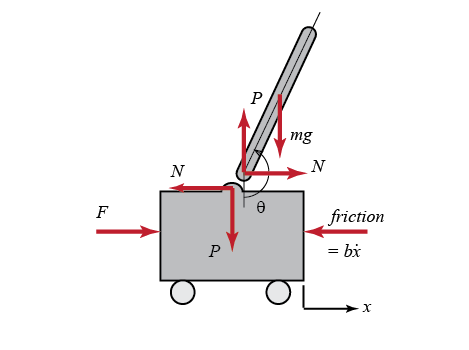
\includegraphics[scale = 0.35]{figs/Selection_045.png} \\

\begin{columns}

\begin{column}{0.45\textwidth}
\scriptsize{
\begin{align*}
\ddot{x}&=\frac{1}{M}\sum_{cart}F_x=\frac{1}{M}(F-N-b\dot{x}) \ &\text{(1)} \\
\ddot{\theta}&=\frac{1}{I}\sum_{pend}\tau=\frac{1}{I}(-Nlcos\theta-Plsin\theta) \ &\text{(2)} \\
N&=m(\ddot{x}-l\dot{\theta}^2sin\theta+l\ddot{\theta}cos\theta) \ &\text{(3)} \\
P&=m(l\dot{\theta}^2 cos\theta+l\ddot{\theta}sin\theta)+g \ &\text{(4)}
\end{align*}
}
\end{column}

\begin{column}{0.5\textwidth}
\tiny{
where \\
\begin{itemize}
\item (M)=mass of the cart=0.5 kg
\item (m)= mass of the pendulum= 0.2 kg
\item (b)=coefficient of friction for cart=0.1 N/m/sec
\item (l)=length to pendulum center of mass=0.3 m
\item (I)= mass moment of inertia of the pendulum= 0.006 kg.$m^2$
\item (F)=force applied to the cart
\item (x)=cart position coordinate 
\item (theta)=pendulum angle from vertical (down)
\end{itemize}
}
\end{column}
\end{columns}

\noindent\makebox[\linewidth]{\rule{10 cm}{0.1pt}}
{\tiny Alternative Quiz}
\href{http://ctms.engin.umich.edu/CTMS/index.php?example=BallBeam&section=SimulinkModeling}{\beamergotobutton{Link}}
\end{frame}

\begin{frame}
\frametitle{Quiz \\ Solution}
\centering
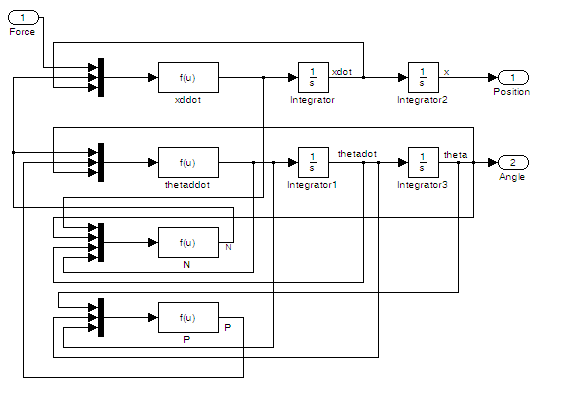
\includegraphics[scale = 0.7]{figs/Selection_046.png} \\
\end{frame}



%%%%%%%%%%%%%%%%


\centering
     \begin{frame}[plain]
           \vspace{2cm}
          \begin{picture}(0,0)(170,170)
          \put(0,0){\includegraphics[width=13 cm,height=9.7 cm]{figs/thank.png}}
         \end{picture}
                  {\huge {Thank you}} % Huge makes the text size, well, Huge
           \vspace{3cm}
           \begin{flushright}
                 \href{mailto:qaziejazurrehman@gmail.com}{\textcolor{white}{Email}}
           \end{flushright}
       \end{frame}
\end{document}
